%%
%% Mosaic paper repository main file.
%%
% TACO submission version.  ACM journals use the acmsmall trim; `review'
% adds the line numbers reviewers are asked to cite, and `anonymous'
% suppresses author names, affiliations, e-mails, and ORCIDs.
% For the camera-ready version, drop `review,anonymous' and restore the
% author block below.
\documentclass[acmsmall,review,anonymous,screen]{acmart}

\AtBeginDocument{%
  \providecommand\BibTeX{{%
    Bib\TeX}}}

% ACM is fully open access; TACO articles are published under CC-BY.
\setcopyright{cc}
\setcctype{by}
\copyrightyear{2026}
\acmYear{2026}
\acmJournal{TACO}
% Volume/number/article/month and the DOI are assigned by ACM at
% acceptance; they stay as placeholders in the submitted version.
\acmVolume{0}
\acmNumber{0}
\acmArticle{0}
\acmMonth{0}
\acmDOI{10.1145/nnnnnnn.nnnnnnn}
% Paste the submission ID issued by Manuscript Central here; it is then
% printed on every page under the `review' option.
\acmSubmissionID{}

% User-defined packages.
\usepackage{xspace}
\usepackage{graphicx}
\usepackage{pgfplots}
\pgfplotsset{compat=1.17}
\usepackage{booktabs}
\usepackage{siunitx}
\usepackage{multirow}
\usepackage{makecell}
\usepackage{adjustbox}
\usepackage{array}
\usepackage{tabularx}
\usepackage{placeins}
\usepackage{enumitem}
\usepgfplotslibrary{statistics, groupplots}
\usetikzlibrary{shapes.geometric, arrows.meta, positioning, fit, backgrounds, positioning, calc, matrix, backgrounds}
\definecolor{primaryblue}{RGB}{70,130,180}
\definecolor{accentorange}{RGB}{255,140,0}
\definecolor{deepgreen}{RGB}{34,139,34}
\definecolor{deepskyblue}{RGB}{46,84,161}
\definecolor{mypurple}{RGB}{112, 48, 160}
\definecolor{lightblue}{RGB}{173, 216, 230}
\definecolor{lightpurple}{RGB}{221, 160, 221}
\definecolor{lightpink}{RGB}{255, 182, 193}
\definecolor{color1}{RGB}{199,56,73}
\definecolor{color2}{RGB}{248,189,211}
\definecolor{color3}{RGB}{191,170,210}
\definecolor{color4}{RGB}{147,197,235}
\definecolor{color5}{RGB}{157,159,163}
\usepackage[utf8]{inputenc}
\usepackage{algorithm}
\usepackage[noend]{algpseudocode}
\usepackage{wrapfig}
% Apply the layout rhythm after acmart installs its document-level defaults.
\AtBeginDocument{%
  % Keep wrapped figures the same distance from the body above and below.
  \setlength{\intextsep}{8pt}%
  \setlength{\textfloatsep}{4pt plus 1pt minus 1pt}%
  \setlength{\floatsep}{8pt plus 2pt minus 2pt}%
  \setlength{\dbltextfloatsep}{8pt plus 2pt minus 2pt}%
  \setlength{\dblfloatsep}{8pt plus 2pt minus 2pt}%
  \setlength{\abovedisplayskip}{4.2pt plus 1pt}%
  \setlength{\belowdisplayskip}{4.2pt plus 1pt}%
  \setlength{\abovedisplayshortskip}{0pt plus 1pt}%
  \setlength{\belowdisplayshortskip}{2.1pt plus 1pt}%
  \setlength{\jot}{4pt}%
}
\usepackage{listings}
\definecolor{darkgray}{rgb}{.3,.3,.3}
\definecolor{darkred}{rgb}{.6,0,0}
\definecolor{darkgreen}{rgb}{0,.6,0}
\definecolor{darkblue}{rgb}{0,0,.6}
\definecolor{codegreen}{rgb}{0,0.6,0}
\definecolor{codegray}{rgb}{0.5,0.5,0.5}
\definecolor{codepurple}{rgb}{0.58,0,0.82}
\definecolor{backcolour}{rgb}{0.95,0.95,0.92}
\lstdefinestyle{patterncode}{
  language=Python,
  basicstyle=\ttfamily\scriptsize,
  keywordstyle=\bfseries\color{black},
  commentstyle=\itshape\color{gray!65},
  stringstyle=\color{black},
  showstringspaces=false,
  breaklines=false,
  frame=single,
  framerule=0.4pt,
  xleftmargin=6pt,
  xrightmargin=6pt,
  aboveskip=2pt,
  belowskip=0pt,
  escapeinside={(*@}{@*)},
  morekeywords={zeros,conv,split,cat,sigmoid,tanh},
}

\newtheorem{definition}{Definition}
\newtheorem{theorem}{Theorem}

\def\sectionautorefname{\S}
\def\subsectionautorefname{\S}
\def\subsubsectionautorefname{\S}
\def\equationautorefname{Eq.}
\def\figureautorefname{Fig.}
\def\tableautorefname{Tab.}
\def\algorithmautorefname{Alg.}
\newcommand{\definitionautorefname}{Def.}
\newcommand{\name}{{Mosaic}\xspace}
\newcommand{\gpu}{GPU\xspace}
\newcommand{\gpus}{GPUs\xspace}
\newcommand{\sm}{SM\xspace}
\newcommand{\sms}{SMs\xspace}
\newcommand{\circled}[1]{\textup{\scriptsize(#1)}}
\newcommand{\tile}{t}
\newcommand{\tvec}{\mathbf{t}}
\newcommand{\rblk}{r}
\newcommand{\rvec}{\mathbf{r}}
\newcommand{\work}{w}
\newcommand{\placement}{\textsc{Placement}\xspace}
\newcommand{\Solve}{\textsc{Solve}}
\newcommand{\Rsm}{R_{\mathrm{SM}}}
\newcommand{\Ssm}{S_{\mathrm{SM}}}
\newcommand{\Sblock}{S_{\mathrm{block}}}
\newcommand{\Bsm}{B_{\mathrm{SM}}}
\newcommand{\Tsm}{T_{\mathrm{SM}}}
\newcommand{\Nsm}{N_{\mathrm{SM}}}
\newcommand{\Tmax}{T_{\max}}
\newcommand{\Wwarp}{w_{\mathrm{warp}}}
\newcommand{\gcoal}{g_{\mathrm{coal}}}
\newcommand{\Lg}{\Lambda_{\mathrm g}}
\newcommand{\Ls}{\Lambda_{\mathrm s}}
\newcommand{\Lr}{\Lambda_{\mathrm r}}
\newcommand{\Lf}{\Lambda_{\mathrm f}}
\newcommand{\Ly}{\Lambda_{\mathrm y}}
\newcommand{\Lglobal}{\Lg}
\newcommand{\Lsmem}{\Ls}
\newcommand{\Lreg}{\Lr}
\newcommand{\Lfma}{\Lf}
\newcommand{\Lsync}{\Ly}
\newcommand{\Czero}{C_0}
\newcommand{\Cinit}{C_{\mathrm{init}}}
\newcommand{\cfma}{c_{\mathrm{fma}}}
\newcommand{\creg}{c_{\mathrm{reg}}}
\newcommand{\Sigmacand}{\Sigma_{\mathrm{cand}}}
% Multi-letter operator name: keep it upright-italic as one token instead of
% the product b*p*s that a bare `bps' typesets as.
\newcommand{\bps}{\mathit{bps}}

% TACO requires an unnumbered footnote on the first page stating the
% relationship of the submission to any prior conference paper.  acmart's
% \titlenote and \thanks both replace their argument with a placeholder under
% the `anonymous' option, so the note is emitted directly instead; it carries
% no author-identifying information and is therefore safe to keep anonymous.
\makeatletter
\newcommand{\firstpagefootnote}[1]{%
  \begingroup
  \renewcommand\thefootnote{}%
  \renewcommand\@makefnmark{}%
  \footnotetext{#1}%
  \addtocounter{footnote}{-1}%
  \endgroup}
\makeatother

% Suppress the page-1 copyright/permission footnote block for this
% submission-stage draft: none of the CC-BY icon+license text, the copyright
% line, the DOI, or the ACM permission-code/article line it prints are
% assigned until acceptance, so showing them here would only display
% placeholders. \setcopyright{cc}/\setcctype{by}/\acmDOI above still record
% the intended camera-ready values; delete this redefinition (restoring
% acmart's default \footnotetextcopyrightpermission) once ACM assigns them.
\makeatletter
\renewcommand\footnotetextcopyrightpermission[1]{}
\makeatother

\begin{document}

% Previous title read as a comparative claim against transformation scheduling
% ("Beyond Schedule Search"), which contradicts the scope statement in
% sec.intro.tex/sec.conclusion.tex: \name operates strictly after scheduling and
% neither searches nor modifies it. Retitled to name the paper's own subject,
% GPU execution space optimization, instead.
% \title{\name: Unified Analytical Optimization of Architecture-Aware GPU Code Generation Beyond Schedule Search}
\title[Analytical Optimization of Architecture-Aware GPU Code Generation]
{Unified Analytical Optimization of Architecture-Aware GPU Execution Space}

\author{Shihan Yuan}
\email{yuanshihan516@hnu.edu.cn}
\orcid{0009-0005-9508-1660}
\author{Junhui Peng}
\email{pengjh0111@hnu.edu.cn}
\orcid{0009-0006-7218-1930}
\author{Guanghui Song}
\email{sheensong@hnu.edu.cn}
\orcid{0009-0001-8089-1151}
\author{Feng Wang}
\email{wangfeng@hnu.edu.cn}
\orcid{0009-0002-4009-6783}
\author{Kenli Li}
\email{lkl@hnu.edu.cn}
\orcid{0000-0002-2635-7716}
\author{Jie Zhao}
\email{jiezhao@hnu.edu.cn}
\orcid{0000-0003-2303-9736}
\affiliation{%
  \institution{Hunan University}
  \city{Changsha}
  \country{China}
}


\begin{abstract}
Selecting tile sizes and thread-block dimensions is critical to the performance of compiler-generated GPU code, yet these choices interact with shared-memory use, register pressure, occupancy, and memory locality. Existing approaches rely on handcrafted heuristics, on analytical models that resolve only some of these interactions, or on empirical search that must be repeated for every new shape and target.

This paper presents \name, a unified analytical framework for GPU execution-space optimization on transformed programs whose schedule and mapping structure have been fixed upstream. \name selects tile and thread-block parameters while reasoning over abstract shared-memory placement scenarios using compiler-provided metadata and a once-per-architecture target profile. Its model combines a quantized wave objective, a shared-read-per-FMA ratio, and a register-working-set consistency filter, followed by a relaxed-cost tie-break among configurations tied at the primary optimum. The formulation also yields a closed-form balanced register-blocking condition for outer-product contractions.

Across 25 PolyBench kernels on three NVIDIA GPUs, \name achieves geometric-mean speedups of $1.21$--$1.49\times$ over PPCG and measured latency ratios of $1.37$--$1.89\times$ relative to EATSS. On the RTX 4090, \name achieves $1.88\times$ over PPCG on deep learning operators and $4.22\times$ over PPCG on end-to-end workloads; on the evaluated end-to-end workloads, it achieves a $1.11\times$ geometric-mean speedup over TVM MetaSchedule. \name further reduces selection overhead by $12$--$14\times$ relative to EATSS and by $2$--$4$ orders of magnitude relative to measurement-driven autotuning.
\end{abstract}

\begin{CCSXML}
<ccs2012>
   <concept>
       <concept_id>10010520.10010521.10010528</concept_id>
       <concept_desc>Computer systems organization~Parallel architectures</concept_desc>
       <concept_significance>500</concept_significance>
       </concept>
   <concept>
       <concept_id>10011007.10011006.10011008</concept_id>
       <concept_desc>Software and its engineering~General programming languages</concept_desc>
       <concept_significance>300</concept_significance>
       </concept>
   <concept>
       <concept_id>10002950.10003624.10003625.10003630</concept_id>
       <concept_desc>Mathematics of computing~Combinatorial optimization</concept_desc>
       <concept_significance>300</concept_significance>
       </concept>
 </ccs2012>
\end{CCSXML}

\ccsdesc[500]{Computer systems organization~Parallel architectures}
\ccsdesc[300]{Software and its engineering~General programming languages}
\ccsdesc[300]{Mathematics of computing~Combinatorial optimization}

\keywords{GPU Code Generation, Execution Space Optimization, Analytical Model, Polyhedral Compilation}

\maketitle

% Mandatory TACO first-page footnote.  Replace with a citation of the prior
% conference paper plus a statement of the >=30% new material if this ever
% becomes an extension rather than a new paper.
\firstpagefootnote{New Paper, Not an Extension of a Conference Paper.}

% !TEX root =  mosaic.tex
\section{Introduction}
\label{sec:intro}

\gpus are the dominant execution platform for scientific computing, machine learning, and data analytics. To target them, modern compilers automatically apply loop transformations such as fusion, distribution, interchange, skewing, and tiling: polyhedral frameworks~\cite{ppcg,pluto,polly,tc,akg} derive these transformations through dependence analysis, while deep learning compilers like Halide~\cite{halide} and TVM~\cite{tvm} expose scheduling primitives that can be explored or tuned.

Transformation scheduling has been extensively explored in these systems, but efficient \gpu code generation also depends on architecture-specific execution parameters that remain after, or are chosen alongside, scheduling. Once a schedule and its mapping structure are fixed, the compiler must still choose tile sizes and thread-block dimensions that govern how the transformed computation consumes shared memory, registers, caches, and streaming multiprocessors (SMs). Unlike loop transformations, which reshape the iteration space and computation order, execution-space optimization leaves them intact and selects resource parameters exposed by the resulting schedule. These decisions therefore complement transformation scheduling rather than replace it.

Prior work on these execution parameters follows two broad lines: analytical selection and empirical search. Analytical tile size selection originated on CPUs, choosing tiles so a footprint stays resident in cache~\cite{mckinley-tss,lam-tss} and later embedding this reasoning in polyhedral~\cite{pluto-tss}, geometric programming~\cite{rajopadhye-gp,rajopadhye-igp}, and decoupled~\cite{tilemind} formulations. \gpu-specific analytical approaches include models derived for individual kernel classes such as matrix multiplication, convolution, or BLAS~\cite{li-gemm,saday-conv,blis}, compiler-integrated tile selection~\cite{ppcg-tss}, and EATSS~\cite{eatss}, which analytically selects \gpu tile sizes under a joint latency--energy objective. Empirical approaches, including autotuners~\cite{metaschedule,ansor,automatichalide} and learning-based pruning~\cite{hctuner,shirako-tss,yuki-tss}, instead explore candidate configurations through measurement or prediction and incur repeated tuning costs for new targets or shapes.

We formulate execution-space selection on a fixed transformed schedule: choosing tile sizes and thread-block dimensions while reasoning over abstract shared-memory placement scenarios and coupled \gpu resource effects. \name uses a compiler-agnostic metadata interface populated by compiler-specific adapters. The execution-space unknowns are coupled: the per-thread register budget depends on the resident-block count, which itself depends on register usage; staging an operand in shared memory cuts global traffic but consumes capacity and can lower the resident-block count; an SM hosts an integer number of blocks, so the grid runs in a discrete number of waves whose boundaries move with tile and placement choices; and the exact register count is fixed by the backend allocator only after code generation.

Our key insight is that these interactions can be captured by two compact quantities whose interaction is what makes the landscape irregular: a \emph{quantized wave cost}, a per-block cost multiplied by an integer wave count, which reproduces the step-function discontinuities that smooth objectives miss, and a \emph{shared-read-per-FMA ratio}, which normalizes operand reads by the arithmetic they serve and exposes register blocking as the lever trading locality against register pressure. Around these, a conservative register-working-set filter rejects only configurations whose register lower bound already exceeds the budget, breaking the occupancy--register cycle by reasoning rather than measurement.

We realize this insight in \name, which operates on the transformed programs emitted by existing schedulers~\cite{ppcg,tvm}. \name selects tile sizes and thread-block dimensions while reasoning over abstract shared-memory placement scenarios and accounting for occupancy and register pressure. It enumerates these scenarios around a two-stage analytical selection with a quantized primary objective and a relaxed-cost tie-break over the Stage-1 optimal discrete configurations, recovering balanced register blocking for outer-product contractions as an analytical outcome rather than an imposed rule. \name sits strictly between transformation scheduling and backend code generation: an upstream compiler first fixes a legal transformation schedule and mapping structure---i.e., which dimensions are assigned to block and thread axes---while \name selects the tile sizes and thread-block dimensions that this structure leaves open. It neither searches nor modifies the schedule or mapping structure. Our current cost model targets conventional CUDA-core SIMT execution, as exercised by the PPCG and non-tensorized TVM paths evaluated in this work; we return to this scope boundary in \autoref{sec:conclusion}.

This distinguishes \name from the prior approaches above: unlike heuristic polyhedral code generation~\cite{ppcg}, it selects execution parameters through an architecture-aware analytical model; unlike kernel-specific \gpu models~\cite{li-gemm,saday-conv,blis}, it spans reductions, contractions, and stencils; unlike prior analytical tile-size selection approaches~\cite{ppcg-tss,eatss,pluto-tss}, it combines placement-aware analytical reasoning with register feasibility and wave quantization; and unlike autotuners~\cite{ansor,metaschedule}, it derives interpretable configurations once, with no per-shape or per-target tuning loop. The evaluation in \autoref{sec:eval} confirms that this analytical reasoning replaces a substantial portion of \gpu execution-space autotuning.

In summary, this work makes the following contributions:
\begin{itemize}
  \item We formulate \gpu execution-space selection as a distinct post-scheduling optimization problem in GPU code generation, complementary to transformation scheduling.
  \item We propose \name, a unified analytical model that selects tile sizes and thread-block dimensions while reasoning over abstract shared-memory placement scenarios and accounting for occupancy and register pressure, closing the coupled feedback loop in one solvable formulation and yielding balanced register blocking as a closed-form optimum for outer-product contractions.
  \item We design a compiler-agnostic analytical core with compiler-specific metadata adapters that operates on transformed programs and integrates with polyhedral schedulers, template-based code generators, and autotuning systems.
  \item We evaluate \name with a cross-generation PolyBench/C~\cite{polybench} study on three NVIDIA \gpus, together with deep learning operators and end-to-end workloads on the RTX 4090, showing aggregate gains over heuristics and analytical selectors and competitive performance with a state-of-the-art autotuner without measurement-driven execution-space search.
\end{itemize}

% !TEX root =  mosaic.tex
\section{Background and Motivation}
\label{sec:background}

This section introduces the background and the GPU-specific challenges behind analytical selection.

\subsection{GPU Execution Space Decisions}
\label{sec:bg-decisions}
\label{sec:gpu-execution-model}

A GPU kernel launches a grid of thread blocks; each block runs on an SM whose resident-block count is limited by block/thread limits, per-block shared memory, and per-thread registers. \name targets the execution space decisions that set these quantities: tile sizes, thread block dimensions, thread mappings, shared memory placement, and register blocking. Larger tiles improve reuse but grow footprint and live state, while smaller tiles raise occupancy but expose less locality. As each tile or placement choice moves several of these limits at once, they cannot be treated as independent dials.

\name does not perform transformation scheduling. It starts from a transformed program whose legal order is fixed by an existing scheduler: schedule trees and affine accesses for polyhedral compilers~\cite{ppcg,tc}, or schedule traces and tensor metadata for template compilers~\cite{halide,tvm}. From this representation, \name extracts loop extents, schedule annotations, access footprints, read/write polarity, operation counts, and coalescing layout, enough to classify dimensions and array roles without depending on compiler internals.


%\subsection{Why Execution Space Parameters Matter}
%\label{sec:bg-why}
%\label{sec:execution space-motivation}

To make the case concrete, we hold one GEMM (general matrix multiplication) schedule fixed and sweep only its execution space parameters: tile sizes \((\tau_i,\tau_j)\), thread block shapes \((b_i,b_j)\), and shared memory placement. We construct 5,000 candidate configurations; 2,232 successfully launched, for which PPCG~\cite{ppcg} emitts each kernel and we measure execution time on an RTX 4090. \autoref{fig:motivation-landscape} plots the results.

\begin{figure}[htbp]
  \centering
  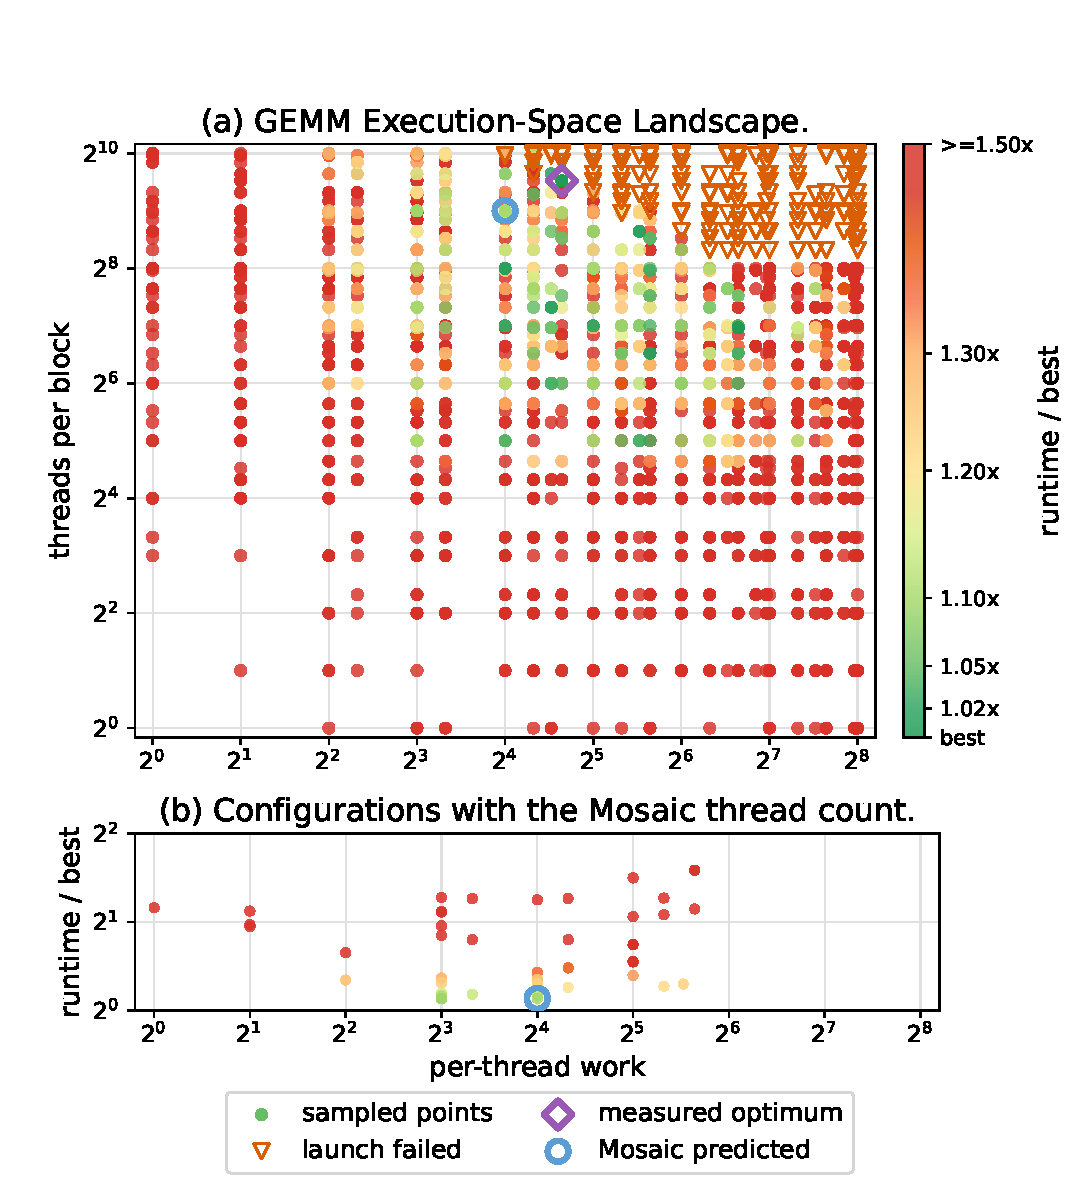
\includegraphics[width=\linewidth]{figure1_main.pdf}
  \caption{GEMM execution space landscape on RTX 4090 under a fixed schedule. (a) Log-ratio runtime for configurations that successfully launch, with measured and predicted optima marked. (b) One-dimensional slice at Mosaic's selected block-thread count, showing measured runtime as a function of per-thread work \(W=R_iR_j\).}
  \Description{Measured performance landscape for GPU GEMM execution space configurations.}
  \label{fig:motivation-landscape}
\end{figure}

\subsection{Transformation-Aware Program Representation}
\label{sec:bg-repr}
\label{sec:program-representation}

Under a single fixed schedule, execution space selection alone moves runtime by more than an order of magnitude, and only 28 of the 2,232 launched configurations (1.25\%) fall within 10\% of the best. Thus the choice of tile size, block shape, and placement, not the schedule, decides performance here. The surface in \autoref{fig:motivation-landscape}(a) is irregular and non-convex, and it shows that \name's analytical selection lands within 10\% of the measured optimum. \autoref{fig:motivation-landscape}(b) fixes the thread block size to the \name-selected block thread count and isolates how per-thread work \(W=R_iR_j\) affects the measured runtime. The slice shows that even after the thread block size is fixed, measured runtime varies substantially with \(W\), so register blocking remains a first-order execution space decision rather than a residual tie break.

\subsection{GPU-Specific Modeling Challenges}
\label{sec:bg-challenges}
\label{sec:gpu-modeling-challenges}

\label{sec:challenge-register-cycle}
\label{sec:challenge-placement}
\label{sec:challenge-discrete-objective}
\label{sec:challenge-register-pressure}

Analytical execution space optimization must address four GPU-specific challenges. First is an occupancy--register circular dependence: the per-thread register budget depends on the number of resident blocks and threads on an SM, yet the resident-block count itself depends in part on register usage, and an analytical model, unlike a tuner, cannot compile each candidate and read back achieved occupancy. Second, shared memory placement is coupled with tile selection: staging read-only operands cuts global traffic but consumes capacity and may lower the resident-block count, so the best placement depends on tile size, block shape, and reuse pattern and cannot be chosen before them. Third is discrete wave quantization: an SM hosts an integer number of blocks, so a grid executes in a discrete number of waves whose ceiling shifts with tile and placement choices, producing step boundaries that no static linear constraint or smooth objective captures. Finally, register pressure is unknown before code generation, because the exact register count is set by the backend allocator afterward, so a sound model needs a conservative compile-time feasibility filter.

The implication is that \emph{these four effects are not independent knobs but one coupled feedback loop}, in which footprint, resident blocks, register budget, and wave count all move together, so they must be resolved jointly in a single formulation rather than by a sequence of independent heuristics.

% !TEX root =  mosaic.tex
\section{Overview of Mosaic}
\label{sec:overview}

\name treats the transformed program as the boundary between transformation
scheduling and execution-space optimization: existing schedulers fix the legal
computation order, and \name decides how that order should consume GPU
architectural resources, emitting tile sizes \(\boldsymbol{\tau}\),
thread-block dimensions \(\mathbf{b}\), and a shared memory placement scheme
\(S\). Throughout, \name operates outside the compiler; the backend is driven
as a black box and all resource reasoning happens in \name. As summarized in
\autoref{fig:mosaic-pipeline}, the workflow comprises four components:

\begin{itemize}
  \item Transformed-program acquisition. \name starts from a program
  whose schedule is already determined by an external compiler. Its loop
  transformations, including fusion, interchange, skewing, distribution, and
  related restructurings, are reflected in the schedule metadata and are neither
  re-derived nor overridden; \name reads schedule-tree annotations for PPCG and
  schedule traces for TVM.
  \item Metadata extraction and target profiling. \name extracts metadata for
  loops, accesses, operations, coalescing, and placement candidates, then
  combines it with once-per-architecture target limits and effective costs,
  yielding the finite execution-space problem instantiated in \autoref{sec:model}.
  \item Analytical execution-space solving. \name enumerates
  shared memory placement schemes for read-only operands and, for each scheme,
  solves over tile sizes and thread-block dimensions; feasibility is checked by
  hardware limits and the conservative register filter, and ranking uses the
  quantized wave cost with an LP tie-break among equal wave costs.
  \item Backend emission. The selected tile sizes, block sizes, and
  placement choices are emitted as backend parameters or CUDA macros.
\end{itemize}

We cast the workflow as a joint minimization over the execution-space candidate
set:
\begin{equation}
(\boldsymbol{\tau}^{*}, \mathbf{b}^{*}, S^{*})
 = \arg\min_{\substack{S \in \Sigma \\
(\boldsymbol{\tau}, \mathbf{b}) \in \mathcal{V}(S)}}
  T_{\mathit{total}}(\boldsymbol{\tau}, \mathbf{b}; S).
\label{eq:two-level}
\end{equation}
Here \(S\) ranges over the power set
\(\Sigma = 2^{\Sigma_{\mathit{cand}}}\) of read-only placement candidates and
\((\boldsymbol{\tau}, \mathbf{b})\) ranges over the placement-dependent feasible
domain \(\mathcal{V}(S)\). \autoref{eq:two-level} is a \emph{single} joint
minimization over the Cartesian product of placements and tile/block choices:
\name solves the inner problem to obtain the best
\((\boldsymbol{\tau}, \mathbf{b})\) cost for \emph{every} placement
\(S \in \Sigma\) and returns the lowest-cost triple overall.
\autoref{sec:metadata} describes the metadata and target profile that
instantiate \autoref{eq:two-level}; \autoref{sec:model} formalizes the cost
model, constraints, and solver.

For the running GEMM example, \name extracts
\(\mathcal{P} = \{i, j\}\), \(\mathcal{R} = \{k\}\), read-only operands \(A\),
\(B\), and register accumulator \(C\), enumerates the induced placement schemes,
solves for tile and block choices, and emits the selected parameters as CUDA
macros.


\begin{figure*}[tbp]
\centering
\resizebox{\textwidth}{!}{%
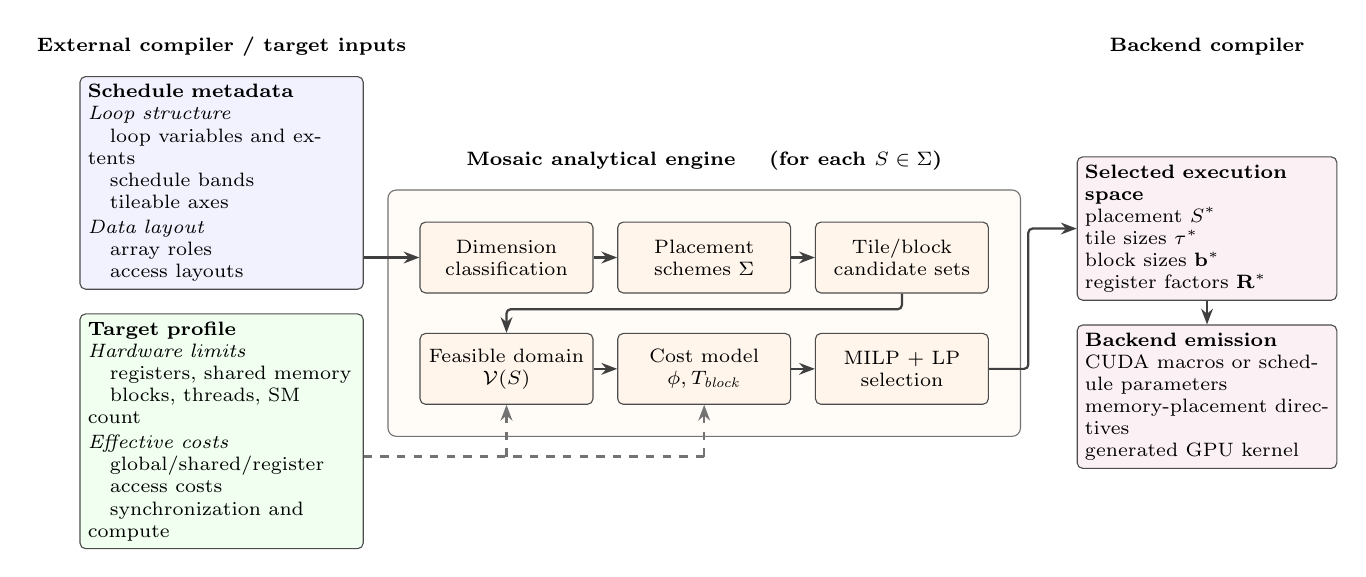
\begin{tikzpicture}[
  font=\scriptsize,
  >={Stealth[length=2mm]},
  box/.style   ={rectangle, rounded corners=2pt, draw=black!70,
                 align=left, inner sep=2.8pt, minimum height=7mm},
  input/.style ={box, fill=blue!5, text width=34mm},
  target/.style={box, fill=green!6, text width=34mm},
  stage/.style ={box, fill=orange!8, align=center, text width=20mm,
                 minimum height=9mm},
  output/.style={box, fill=purple!6, text width=31mm},
  title/.style ={font=\scriptsize\bfseries, align=center},
  arr/.style   ={->, thick, draw=black!75},
  darr/.style  ={->, thick, dashed, draw=black!55},
  dline/.style ={thick, dashed, draw=black!55},
]

\node[input] (sched) {%
\textbf{Schedule metadata}\\
\textit{Loop structure}\\
\quad loop variables and extents\\
\quad schedule bands\\
\quad tileable axes\\[1pt]
\textit{Data layout}\\
\quad array roles\\
\quad access layouts};

\node[target, below=3mm of sched] (prof) {%
\textbf{Target profile}\\
\textit{Hardware limits}\\
\quad registers, shared memory\\
\quad blocks, threads, SM count\\[1pt]
\textit{Effective costs}\\
\quad global/shared/register\\
\quad access costs\\
\quad synchronization and compute};

\begin{scope}[on background layer]
  \node[fit=(sched)(prof), inner sep=0pt] (inputgroup) {};
\end{scope}

\node[title, anchor=south]
      (inputtitle)
      at ([yshift=1.2mm]inputgroup.north)
      {External compiler / target inputs};

\node[stage, anchor=west]
      (cls)
      at ([xshift=7mm,yshift=7mm]inputgroup.east)
      {Dimension\\classification};

\node[stage, right=3mm of cls]
      (plc)
      {Placement\\schemes \(\Sigma\)};

\node[stage, right=3mm of plc]
      (cand)
      {Tile/block\\candidate sets};

\node[stage, below=5mm of cls]
      (feas)
      {Feasible domain\\\(\mathcal{V}(S)\)};

\node[stage, right=3mm of feas]
      (cost)
      {Cost model\\\(\phi,T_{\mathit{block}}\)};

\node[stage, right=3mm of cost]
      (solve)
      {MILP + LP\\selection};

\begin{scope}[on background layer]
  \node[
    draw=black!55,
    rounded corners=3pt,
    fill=orange!3,
    inner xsep=4mm,
    inner ysep=4mm,
    fit=(cls)(plc)(cand)(feas)(cost)(solve)
  ] (engine) {};
\end{scope}

\node[title, anchor=south]
      at ([yshift=1.2mm]engine.north)
      {\textsc{Mosaic} analytical engine
       \quad (for each \(S\in\Sigma\))};

\draw[arr] (cls.east) -- (plc.west);
\draw[arr] (plc.east) -- (cand.west);

\draw[arr, rounded corners=1.5pt]
  (cand.south) -- ++(0,-2mm) -| (feas.north);

\draw[arr] (feas.east) -- (cost.west);
\draw[arr] (cost.east) -- (solve.west);

\coordinate (schedexit) at (sched.east |- cls.west);
\draw[arr] (schedexit) -- (cls.west);

\coordinate (profileleft)
  at ([yshift=-2.5mm]engine.south west);

\coordinate (profilefeas)
  at (feas.south |- profileleft);

\coordinate (profilecost)
  at (cost.south |- profileleft);

\coordinate (profexit)
  at (prof.east |- profileleft);

\draw[dline] (profexit) -- (profilecost);
\draw[darr] (profilefeas) -- (feas.south);
\draw[darr] (profilecost) -- (cost.south);

\matrix (backendboxes) [
  matrix,
  anchor=west,
  row sep=3mm,
  inner sep=0pt
] at ([xshift=7mm]engine.east |- inputgroup.center) {

  \node[output] (out) {%
    \textbf{Selected execution space}\\
    placement \(S^{*}\)\\
    tile sizes \(\boldsymbol{\tau}^{*}\)\\
    block sizes \(\mathbf{b}^{*}\)\\
    register factors \(\mathbf{R}^{*}\)}; \\

  \node[output] (gen) {%
    \textbf{Backend emission}\\
    CUDA macros or schedule parameters\\
    memory-placement directives\\
    generated GPU kernel}; \\
};

\node[title, anchor=center]
      at (backendboxes.north |- inputtitle.center)
      {Backend compiler};

\draw[arr, rounded corners=1.5pt]
  (solve.east) -- ++(5mm,0) |- (out.west);

\draw[arr] (out.south) -- (gen.north);

\end{tikzpicture}}
\caption{Workflow of \textsc{Mosaic}. An external compiler or scheduler supplies
schedule metadata, while the target profile supplies architecture limits and
effective costs. \textsc{Mosaic} classifies dimensions, enumerates placements,
constructs candidates, filters feasibility, models cost, and performs MILP+LP
selection. The backend consumes the selected tile sizes, block dimensions, and
memory-placement directives to emit GPU code; no candidate kernel is generated
or timed during selection.}
\Description{Compact workflow diagram separating compiler inputs, the Mosaic
analytical engine, and backend code emission.}
\label{fig:mosaic-pipeline}
\end{figure*}

\name is realized as a backend-agnostic Python pipeline that consumes schedule
information, runs the analytical selection of \autoref{sec:model} outside the
compiler, and returns the chosen configuration as code-generation parameters.
It treats the schedule as an abstraction layer rather than reaching into
compiler internals: from it \name extracts the loop flags, affine access maps,
tile footprints, read/write polarities, and operation counts required by the
model, from which the program-derived quantities \(\dim(A)\),
\(K_{\mathit{total}}\), tile footprints, and stencil halo widths \(h_d\) follow
directly. The same engine drives both backends and reads identical fields from
each: PPCG exposes this information through schedule trees, and TVM through
schedule traces. For every placement scheme it assembles the Stage-1 MILP and
Stage-2 LP of \autoref{eq:two-level}, solved with PuLP and the CBC backend, and
keeps the lowest-cost scheme. The selected tiles, block dimensions, and staged
operands are emitted as backend configuration parameters, including shared memory
buffers with cooperative loads and barriers for PPCG, schedule parameters for
TVM, while capacity parameters come from device properties and the effective
\(L\)/\(c\) constants from the microbenchmarks of
\autoref{sec:gpu-target-profiling}. Because all resource reasoning happens
outside the backend, no candidate kernel is generated or timed during selection.

% !TEX root =  mosaic.tex
\section{Metadata Extraction and GPU Profiling}
\label{sec:metadata}

This section explains how \name converts a transformed program and a target \gpu into the constants required by \autoref{eq:two-level}. \name instantiates its analytical model from two sources: compile-time metadata extracted from the transformed program and target-specific constants obtained once per \gpu architecture. The first source describes the computation and its transformed loop structure; the second describes the resource limits and effective costs of the target. Together, they determine the candidate variables, resource footprints, feasibility constraints, and cost terms used by the solver.

\subsection{Compile-Time Metadata}
\label{sec:compile-time-metadata}

The transformed representation exposes the loop order and mapping decisions the scheduler already made, so \name optimizes execution space parameters without redoing them.

The metadata falls into several groups tied to the model. These groups are chosen to capture the information the cost model requires: loop structure drives candidate generation, array metadata drives traffic and placement decisions, statement metadata drives compute and synchronization cost, and GPU-specific mapping metadata closes the occupancy and register loop. Loop structure records dimension names, bounds, schedule order, and step sizes; with \(N_d\) the extent of dimension \(d\), these define the tile and block candidate sets. Dimension annotations record permutable and coincident (i.e., parallelizable) dimensions, from which \name classifies each loop as parallel (\(\mathcal{P}\), mappable to independent blocks/threads), reduction (\(\mathcal{R}\), absent from every write footprint), or serial (\(\mathcal{D}\), neither of the former); the formal definition is \autoref{eq:dimension-roles} in \autoref{sec:abstraction}. Array metadata records affine accesses, read/write polarity, layout, coalescing direction, and tile footprints, determining memory traffic, shared memory capacity, accumulator placement, and staging candidates. Statement metadata records arithmetic counts, memory-reference counts, and synchronization sites, which instantiate compute and barrier costs. GPU-specific mapping metadata adds block/thread mappings, shared memory staging candidates, register-blocking factors \(\rblk_d=\tile_d/b_d\), and coalescing.

The shared memory placement candidates are restricted to read-only references whose tile footprints are functions of the candidate tile sizes; \autoref{tab:placement-rules} assigns every other reference a fixed memory space. This restriction keeps the outer enumeration small while retaining the placements that materially affect reuse, shared memory footprint, and occupancy.

\begin{table}[htbp]
  \caption{Placement rules.}
  \label{tab:placement-rules}
  \centering
  \scriptsize
  \setlength{\tabcolsep}{0pt}
  \renewcommand{\arraystretch}{1.05}

  \begin{tabularx}{\columnwidth}{
    @{}
    >{\raggedright\arraybackslash}X
    @{}
  }
    \toprule
    \textbf{Array polarity and placement decision} \\
    \midrule

    \textbf{Read/write accumulators.}\par
    Place in registers to keep private accumulated outputs
    close to the thread. \\

    \addlinespace[2.5pt]

    \textbf{Write-only coalesced references.}\par
    Keep in global memory and stream the output directly. \\

    \addlinespace[2.5pt]

    \textbf{Write-only uncoalesced or transposed references.}\par
    Use shared memory to restore coalescing before global
    writeback. \\

    \addlinespace[2.5pt]

    \textbf{Read-only references.}\par
    Form \(\Sigma_{\mathit{cand}}\); the cost model decides
    whether staging is profitable. \\

    \bottomrule
  \end{tabularx}
\end{table}

\autoref{fig:gemm-schedule-metadata} illustrates metadata construction using the default PPCG schedule of the running GEMM example and the dimension sets defined in \autoref{eq:dimension-roles}. In general, \name requires only the categories above; polyhedral compilers expose them through schedule trees and affine access maps, while TVM-style compilers expose them through schedule traces and tensor access metadata.

% Figure palette
\definecolor{color1}{RGB}{199,56,73}
\definecolor{color2}{RGB}{248,189,211}
\definecolor{color3}{RGB}{191,170,210}
\definecolor{color4}{RGB}{147,197,235}
\definecolor{color5}{RGB}{157,159,163}

\definecolor{color1}{RGB}{199,56,73}
\definecolor{color2}{RGB}{248,189,211}
\definecolor{color3}{RGB}{191,170,210}
\definecolor{color4}{RGB}{147,197,235}
\definecolor{color5}{RGB}{157,159,163}

\begin{figure}[htbp]
\centering
% \setlength{\abovecaptionskip}{10pt}
\resizebox{0.96\columnwidth}{!}{%
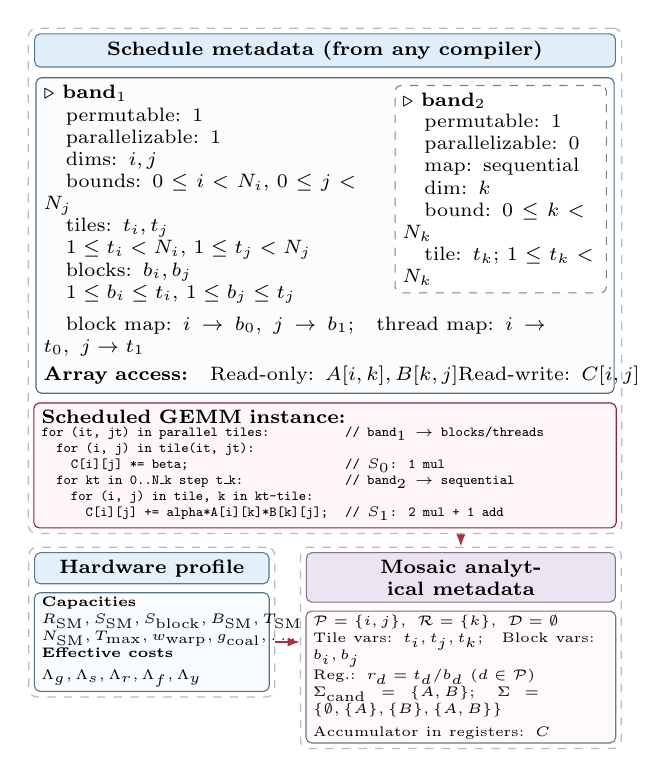
\begin{tikzpicture}[
  font=\scriptsize,
  box/.style={
    draw=color5!82!black,
    fill=white,
    rounded corners=2pt,
    inner sep=2.6pt,
    text width=#1,
    align=left
  },
  textonly/.style={
    text width=#1,
    align=left,
    inner sep=0pt
  },
  hdr/.style={
    draw=color5!82!black,
    rounded corners=2pt,
    inner sep=2.5pt,
    fill=color5!12,
    font=\scriptsize\bfseries,
    align=center
  },
  arr/.style={
    -{Latex[length=1.55mm]},
    line width=0.55pt,
    draw=color1!85!black
  },
  grpborder/.style={
    draw=color5!72,
    rounded corners=3pt,
    line width=0.45pt,
    dashed
  },
]

\node[
  hdr,
  text width=72mm,
  fill=color4!30,
  draw=color4!62!black
] (src_hdr) at (0,0)
  {Schedule metadata (from any compiler)};

\node[
  textonly=41mm,
  anchor=north west
] (bandone_text)
  at ([xshift=-35.8mm,yshift=-2.2mm]src_hdr.south)
{%
  \(\triangleright\) \textbf{band\(_1\)}\\
  \quad permutable: 1\\
  \quad parallelizable: 1\\
  \quad dims: \(i,j\)\\
  \quad bounds: \(0\le i<N_i\), \(0\le j<N_j\)\\
  \quad tiles: \(t_i,t_j\)\\
  \quad \(1\le t_i<N_i\), \(1\le t_j<N_j\)\\
  \quad blocks: \(b_i,b_j\)\\
  \quad \(1\le b_i\le t_i\), \(1\le b_j\le t_j\)
};

\node[
  box=25mm,
  dashed,
  anchor=north east
] (bandtwo_box)
  at ([xshift=35.8mm,yshift=-2.2mm]src_hdr.south)
{%
  \(\triangleright\) \textbf{band\(_2\)}\\[-0.2pt]
  \quad permutable: 1\\
  \quad parallelizable: 0\\
  \quad map: sequential\\
  \quad dim: \(k\)\\
  \quad bound: \(0\le k<N_k\)\\
  \quad tile: \(t_k\); \(1\le t_k<N_k\)
};

\node[
  textonly=68mm,
  anchor=north west
] (mapping_text)
  at ([xshift=0mm,yshift=-1.5mm]bandone_text.south west)
{%
  \quad block map: \(i\to b_0,\ j\to b_1\);\quad
  thread map: \(i\to t_0,\ j\to t_1\)
};

\node[
  textonly=68mm,
  anchor=north west
] (access_text)
  at ([xshift=0mm,yshift=-1.15mm]mapping_text.south west)
{%
  \makebox[\linewidth][l]{%
    \textbf{Array access:}\quad
    Read-only: \(A[i,k],B[k,j]\)\hfill
    Read-write: \(C[i,j]\)}
};

\begin{scope}[on background layer]
  \node[
    draw=color4!55!black,
    fill=color4!5,
    rounded corners=2pt,
    inner sep=2.6pt,
    fit=(bandone_text)(bandtwo_box)(mapping_text)(access_text)
  ] (loop_box) {};
\end{scope}

\node[
  box=72mm,
  draw=color1!68!black,
  fill=color2!13,
  anchor=north,
  inner xsep=2.8pt,
  inner ysep=2.5pt
] (code_box)
  at ([yshift=-1.1mm]loop_box.south)
{%
  \textbf{Scheduled GEMM instance:}\\[-0.2pt]
  {\ttfamily\fontsize{4.75pt}{5.75pt}\selectfont
  \begin{tabular}{@{}l@{\hspace{1.15em}}l@{}}
  for (it, jt) in parallel tiles:
    & // band$_1$ $\to$ blocks/threads\\
  \quad for (i, j) in tile(it, jt):
    & \\
  \qquad C[i][j] *= beta;
    & // $S_0$: 1 mul\\
  \quad for kt in 0..N\_k step t\_k:
    & // band$_2$ $\to$ sequential\\
  \qquad for (i, j) in tile, k in kt-tile:
    & \\
  \qquad\quad C[i][j] += alpha*A[i][k]*B[k][j];
    & // $S_1$: 2 mul + 1 add
  \end{tabular}}
};

\coordinate (lower_top)
  at ([yshift=-3.0mm]code_box.south);
\node[
  hdr,
  text width=28mm,
  fill=color4!24,
  draw=color4!62!black,
  anchor=north west
] (hw_hdr)
  at ([xshift=0mm]src_hdr.west |- lower_top)
  {Hardware profile};

\node[
  box=28mm,
  draw=color4!58!black,
  fill=color4!6,
  anchor=north,
  yshift=-1.0mm,
  minimum height=12.0mm,
  inner ysep=1.5pt
] (hw_box)
  at (hw_hdr.south)
{%
  {\fontsize{5.15pt}{6.15pt}\selectfont
  \textbf{Capacities}\\
  \(R_{\mathrm{SM}},
    S_{\mathrm{SM}},
    S_{\mathrm{block}},
    B_{\mathrm{SM}},
    T_{\mathrm{SM}}\)\\
  \(N_{\mathrm{SM}},
    T_{\max},
    w_{\mathrm{warp}},
    g_{\mathrm{coal}},
    \ldots\)\\
  \textbf{Effective costs}\\
  \(\Lambda_g,
    \Lambda_s,
    \Lambda_r,
    \Lambda_f,
    \Lambda_y\)}
};

\begin{scope}[on background layer]
  \node[
    grpborder,
    inner sep=1.8pt,
    fit=(hw_hdr)(hw_box)
  ] (hw_grp) {};
\end{scope}

\node[
  hdr,
  text width=37.5mm,
  fill=color3!32,
  draw=color3!68!black,
  anchor=north east
] (out_hdr)
  at ([xshift=0mm]src_hdr.east |- lower_top)
  {\name analytical metadata};

\node[
  box=37.5mm,
  draw=color3!64!black,
  fill=color2!9,
  anchor=north,
  yshift=-1.0mm,
  minimum height=12.0mm,
  inner ysep=1.5pt
] (out_box)
  at (out_hdr.south)
{%
  {\fontsize{5.15pt}{6.15pt}\selectfont
  \(\mathcal P=\{i,j\},\
    \mathcal R=\{k\},\
    \mathcal D=\emptyset\)\\
  Tile vars: \(t_i,t_j,t_k\);\quad
  Block vars: \(b_i,b_j\)\\
  Reg.: \(r_d=t_d/b_d\ (d\in\mathcal P)\)\\
  {\fontsize{4.55pt}{6.15pt}\selectfont
  \(\Sigma_{\mathrm{cand}}=\{A,B\};\quad
    \Sigma=\{\emptyset,\{A\},\{B\},\{A,B\}\}\)}\\
  Accumulator in registers: \(C\)}
};

\begin{scope}[on background layer]
  \node[
    grpborder,
    inner sep=1.8pt,
    fit=(out_hdr)(out_box)
  ] (out_grp) {};
\end{scope}

\begin{scope}[on background layer]
  \node[
    grpborder,
    inner sep=1.8pt,
    fit=(src_hdr)(loop_box)(code_box)
  ] (sched_grp) {};
\end{scope}

\coordinate (sched_arrow_start)
  at (out_grp.north |- sched_grp.south);

\draw[arr]
  (sched_arrow_start)
  -- (out_grp.north);

\coordinate (hw_exit)
  at (hw_grp.east |- hw_box.center);

\coordinate (hw_entry)
  at (out_grp.west |- hw_box.center);

\draw[arr]
  (hw_exit)
  -- (hw_entry);

\end{tikzpicture}%
}

\caption{
  GEMM metadata construction.
  Schedule metadata from the PPCG schedule tree, combined with a
  one-time hardware profile, yields the \name analytical metadata,
  with the dimension sets following \autoref{eq:dimension-roles}.
}

\Description{
  A compact single-column flow diagram in which a rectangular
  schedule-metadata panel contains a GEMM schedule-tree instance,
  while a one-time hardware profile and the schedule metadata feed
  \name analytical metadata.
}

\label{fig:gemm-schedule-metadata}
\end{figure}

In this example, the dimension sets defined in \autoref{eq:dimension-roles} give \(\mathcal{P}=\{i,j\}\), which creates \(\tile_i,\tile_j\) and \(b_i,b_j\); \(\mathcal{R}=\{k\}\), which creates \(\tile_k\) but no block dimension. The register-blocking factors \(\rblk_i=\tile_i/b_i\) and \(\rblk_j=\tile_j/b_j\) follow from these tile and block choices rather than entering as separate variables. The read-only operands give \(\Sigma_{\mathit{cand}}=\{A,B\}\), whose four binary-based placement schemes change the footprint, traffic, and resident-block bound used in \autoref{sec:model}.

\subsection{GPU Target Profiling}
\label{sec:gpu-target-profiling}

The target description combines hardware constants queried from the device with effective costs measured once per architecture and reused across all kernels for that target. The hardware constants, including SM count, warp size, resident block and thread limits, shared memory capacities, register-file size, and block-size limit (\autoref{tab:model-notation}), bound the resident-block count, occupancy, and feasible domain. The effective costs, the \(\Lambda\)-family constants of \autoref{tab:model-notation}, come from targeted microbenchmarks and enter the matching terms of \(T_{\mathit{block}}\). They serve relative ranking and analytical selection, not cycle-accurate prediction; the model captures the resource interactions that shape the execution space landscape and leaves backend scheduling, caching, and pipeline overlap as lower-level effects.

\begin{table}[htbp]
  \caption{Model notation.}
  \label{tab:model-notation}
  \centering
  \scriptsize
  \setlength{\tabcolsep}{3pt}
  \begin{tabular}{p{0.30\linewidth}p{0.59\linewidth}}
    \toprule
    Symbol & Meaning \\
    \midrule
    \multicolumn{2}{l}{\textbf{Decision variables}} \\[1pt]
    \(\tile_d,\ b_d,\ \rblk_d\) & Tile size, thread-block size, and per-thread
                              register-blocking factor for dimension~\(d\). \\
    \(\work,\ S \in \Sigma\)   & Per-thread output count; shared memory
                              placement scheme (subset of \(\Sigma_{\mathit{cand}}\)). \\
    \midrule
    \multicolumn{2}{l}{\textbf{Architecture constants}
      \textit{(queried or profiled once per GPU)}} \\[1pt]
    \(\Nsm,\Bsm,\Tsm,\Tmax\) &
      SM count; max resident blocks and threads per SM; max threads per block. \\
    \(\Ssm,\Sblock,\Rsm\) &
      Per-SM and per-block shared memory capacity; SM register-file size. \\
    \(\Lg,\Ls,\Lf,\Ly\) &
      Effective costs for global access, shared-memory access, FMA,
      and barrier synchronization. \\
    \(\Lr,\ \gcoal\) &
      Register-access cost; coalescing granularity for loads. \\
    \midrule
    \multicolumn{2}{l}{\textbf{Key derived quantities}} \\[1pt]
    \(\phi_{\square}\) &
      Reads-per-FMA ratio for placement class
      \(\square\!\in\!\{\mathit{smem},\mathit{gmem}\}\);
      links register blocking to memory traffic in \(T_{\mathit{compute}}\). \\
    \(\operatorname{smem}(\tvec;S),\ |A|_{\tvec}\) &
      Shared-memory footprint and operand tile footprint. \\
    \(K_{\mathit{outer}}\) &
      Cooperative load rounds \(\prod_{r\in\mathcal{R}}\lceil N_r/\tile_r\rceil\)
      over tiled reduction dimensions. \\
    \(bps,\ R_{\mathit{avail}},\ \hat{R}\) &
      Resident blocks per SM; available registers per thread;
      conservative register working-set estimate. \\
    \bottomrule
  \end{tabular}
\end{table}

In practice, the microbenchmark suite is fewer than ten short kernels, each measuring one cost constant in isolation, and completes in under two minutes on any of the three GPUs. The profiled constants depend only on the architecture, not on any kernel or problem size, so this one-time cost amortizes across all kernels for that target.

% !TEX root =  mosaic.tex
\section{Analytical Modeling and Problem Solving}
\label{sec:model}

Given transformed metadata and target constants, \name selects tile sizes \(\tvec\), thread block dimensions \(\mathbf{b}\), and placement scheme \(S\), inducing register-blocking factors \(\rblk_d=\tile_d/b_d\), footprints, resident blocks, waves, and register working sets; \autoref{tab:model-notation} summarizes the main notation. Recall from \autoref{eq:two-level} that the joint minimization over \(S\) and \((\tvec,\mathbf{b})\) factorizes into an outer placement enumeration and, for each fixed \(S\), an inner minimization. The inner objective is the quantized wave cost.
\begin{equation}
\min_{\tvec,\mathbf{b},S}
T_{\mathit{block}}(\tvec,\mathbf{b};S)
\cdot
\left\lceil
\dfrac{N_{\mathit{blocks}}(\tvec)}
      {\Nsm \cdot bps(\tvec,\mathbf{b};S)}
\right\rceil,
\label{eq:model-summary}
\end{equation}
Here \(bps\) is the resident blocks per \sm (\autoref{eq:resident-blocks}) and \(T_{\mathit{block}}\) is the per-block cost (\autoref{eq:block-cost}); \autoref{eq:model-summary} is thus the inner form of \autoref{eq:two-level}, and the outer loop selects the placement with the lowest inner optimum. The objective is subject to thread/block limits, minimum useful parallelism, shared-memory capacity, and register feasibility (\autoref{eq:feasible-domain}).

\subsection{Candidate Space}
\label{sec:abstraction}
\label{sec:placement}

From the metadata of \autoref{sec:metadata}, each loop dimension is labeled according to its role in the transformed schedule. Parallel dimensions are those that can be legally mapped to independent thread blocks and threads; reduction dimensions are those absent from all write footprints, meaning their iterations produce partial results that must be accumulated; serial dimensions are those that are neither parallel nor reduction and must execute sequentially within each thread. Formally:
\begin{equation}
\begin{aligned}
\mathcal{P}
&= \{d \mid \mathit{parallelizable}[d] = 1\},\\
\mathcal{R}
&= \{d \notin \mathcal{P}
    \mid d \notin \dim(A)\ \text{for every written array } A\},\\
\mathcal{D}
&= \{d \mid d\notin\mathcal{P},\ d\notin\mathcal{R}\}.
\end{aligned}
\label{eq:dimension-roles}
\end{equation}
\(\mathit{parallelizable}[d]=1\) denotes a dimension that can legally execute in parallel; for polyhedral schedules this includes coincident dimensions with no carried dependence, and TVM axes bound to CUDA block or thread indices are treated analogously. Reduction axes populate \(\mathcal{R}\), and serial dimensions remain untiled. Serial dimensions \(\mathcal{D}\) are those belonging to neither \(\mathcal{P}\) nor \(\mathcal{R}\); they remain at their full loop extents, are not assigned tile or block variables, and do not contribute to the candidate generation of \autoref{eq:tile-candidates}. For GEMM, \(\mathcal{D}=\emptyset\).

Parallel dimensions map to thread and block indices, while reduction dimensions contribute only to per-output work \(K_{\mathit{total}}\). The reduction work per output element is a compile-time constant independent of any tile choice:
\begin{equation}
K_{\mathit{total}} = \prod_{r \in \mathcal{R}} N_r.
\label{eq:reduction-work}
\end{equation}

\name builds a discrete tile candidate set from powers of two and exact divisors:
\begin{equation}
C_d
= \{2^k \mid 2^k < N_d\}
  \cup \{v \mid v \text{ divides } N_d\}.
\label{eq:tile-candidates}
\end{equation}
Powers of two align tiles with the warp size and coalescing granularity, while exact divisors of \(N_d\) eliminate boundary-remainder loops and partial waves; arbitrary tile sizes are excluded since they neither improve coalescing nor divide the extent evenly, yet would enlarge the candidate space combinatorially. For each \(\tile_d\in C_d\), block candidates are restricted to divisors of \(\tile_d\), keeping
\(\rblk_d=\tile_d/b_d\) integral; hardware limits are imposed later.

Each array is assigned a memory space from its read/write polarity
(\autoref{tab:placement-rules}). Read-only operands form
\(\Sigma_{\mathit{cand}}\), and \name enumerates
\(\Sigma=2^{\Sigma_{\mathit{cand}}}\) during solving of
\autoref{eq:two-level}. Accumulators and ordinary write-only references are
excluded, keeping the placement space small.

\begin{table}[htbp]
  \caption{Model notation.}
  \label{tab:model-notation}
  \centering
  \scriptsize
  \setlength{\tabcolsep}{3pt}
  \begin{tabular}{p{0.30\linewidth}p{0.59\linewidth}}
    \toprule
    Symbol & Meaning \\
    \midrule
    \multicolumn{2}{l}{\textbf{Decision variables}} \\[1pt]
    \(\tile_d,\ b_d,\ \rblk_d\) & Tile size, thread-block size, and per-thread
                              register-blocking factor for dimension~\(d\). \\
    \(\work,\ S \in \Sigma\)   & Per-thread output count; shared memory
                              placement scheme (subset of \(\Sigma_{\mathit{cand}}\)). \\
    \midrule
    \multicolumn{2}{l}{\textbf{Architecture constants}
      \textit{(queried or profiled once per GPU)}} \\[1pt]
    \(\Nsm,\Bsm,\Tsm,\Tmax\) &
      SM count; max resident blocks and threads per SM; max threads per block. \\
    \(\Ssm,\Sblock,\Rsm\) &
      Per-SM and per-block shared memory capacity; SM register-file size. \\
    \(\Lg,\Ls,\Lf,\Ly\) &
      Effective costs for global access, shared-memory access, FMA,
      and barrier synchronization. \\
    \(\Lr,\ \gcoal\) &
      Register-access cost; coalescing granularity for loads. \\
    \midrule
    \multicolumn{2}{l}{\textbf{Key derived quantities}} \\[1pt]
    \(\phi_{\square}\) &
      Reads-per-FMA ratio for placement class
      \(\square\!\in\!\{\mathit{smem},\mathit{gmem}\}\);
      links register blocking to memory traffic in \(T_{\mathit{compute}}\). \\
    \(\operatorname{smem}(\tvec;S),\ |A|_{\tvec}\) &
      Shared-memory footprint and operand tile footprint. \\
    \(K_{\mathit{outer}}\) &
      Cooperative load rounds \(\prod_{r\in\mathcal{R}}\lceil N_r/\tile_r\rceil\)
      over tiled reduction dimensions. \\
    \(bps,\ R_{\mathit{avail}},\ \hat{R}\) &
      Resident blocks per SM; available registers per thread;
      conservative register working-set estimate. \\
    \bottomrule
  \end{tabular}
\end{table}

Equivalently, the joint execution space candidate set is \(\prod_{d\in\mathcal{P}\cup\mathcal{R}} C_d \times \Sigma\), with each \(\tile_d\in C_d\) paired with divisor choices for admissible block dimensions; \(\mathcal{V}(S)\) then filters this product to legal configurations for the objective of \autoref{eq:two-level}.

Following the placement rules in \autoref{tab:placement-rules}, for a fixed \(S\), let \(\mathcal{A}_{\mathit{smem}}=S\) and \(\mathcal{A}_{\mathit{gmem}}=\Sigma_{\mathit{cand}}\setminus S\). With \(\work=\prod_{d\in\mathcal{P}}\rblk_d\) outputs per thread, the induced resource quantities used by the constraints and cost model are the shared memory footprint \(\operatorname{smem}(\tvec;S)\), the read counts \(R^{\mathit{smem}}_{\mathit{in}}\) and \(R^{\mathit{gmem}}_{\mathit{in}}\), and the register working set \(\hat{R}\). The per-reduction-step read count and its normalized ratio are
\begingroup
\small
\begin{equation}
\begin{aligned}
R^{\square}_{\mathit{in}}
&= \sum_{A \in \mathcal{A}_{\square}}
   \prod_{d \in \dim(A) \cap \mathcal{P}} \rblk_d,\\
\phi_{\square}
&= \dfrac{R^{\square}_{\mathit{in}}}{\work}
 = \sum_{A \in \mathcal{A}_{\square}}
   \prod_{d \in \mathcal{P} \setminus \dim(A)} \rblk_d^{-1},
   \qquad \square \in \{\mathit{smem},\mathit{gmem}\}.
\end{aligned}
\label{eq:read-ratios}
\end{equation}
\endgroup

For the GEMM example with both operands staged (\(\mathcal{P}=\{i,j\}\), \(\mathcal{R}=\{k\}\), \(\Sigma_{\mathit{cand}}=\{A,B\}\); \autoref{fig:gemm-schedule-metadata}), \autoref{eq:read-ratios} gives \(\work=\rblk_i\rblk_j\) outputs per thread and \(\phi_{\mathit{smem}}=\rblk_i^{-1}+\rblk_j^{-1}\).

\subsection{Feasibility Constraints}
\label{sec:constraints}
\label{sec:register-filter}

The inner feasible domain \(\mathcal{V}(S)\) is the set of tile/block choices that, for a fixed placement \(S\), satisfy every launch and resource constraint; it is the domain over which the inner objective (\autoref{eq:model-summary}) is minimized, after which the outer loop compares the optima across placements (\autoref{eq:two-level}). It collects launch limits and pruning rules:
\begin{equation}
\begin{gathered}
\mathcal{V}(S)
= \{(\tvec,\mathbf{b}) \mid \text{C1--C4 hold}\},\\[0.6ex]
\begin{array}{@{}l@{\qquad}l@{}}
\text{C1: } \displaystyle \prod_{d\in\mathcal{P}} b_d \le \Tmax
&
\text{C2: } \displaystyle \prod_{d\in\mathcal{P}} b_d \ge \Wwarp
\\[2.8ex]
\text{C3: } \operatorname{smem}(\tvec;S)\le \Sblock
&
\text{C4: } \hat{R}\le R_{\mathit{avail}}.
\end{array}
\end{gathered}
\label{eq:feasible-domain}
\end{equation}
C1 and C2 enforce block-size legality and useful parallelism; C3 bounds placement-dependent shared memory; C4 is the conservative register filter.

The register filter breaks the occupancy and register circular dependence by ordering the quantities in one direction; the symbols used below are summarized in \autoref{tab:model-notation}. First, \name ignores the register constraint and computes a pre-register resident-block bound from the block limit, thread limit, and shared memory usage. This gives \(bps\). Second, \(bps\) and the number of threads per block determine the available register budget per thread, \(R_{\mathit{avail}}\). Third, a conservative working set estimate \(\hat{R}\) is checked against that budget:
\begingroup
\renewcommand{\arraystretch}{1.12}
\begin{equation}
\begin{array}{@{}l@{\;}l@{}}
bps
&= \min\left(
   \Bsm,
   \left\lfloor \dfrac{\Tsm}{\prod_{d\in\mathcal{P}} b_d} \right\rfloor,
   \left\lfloor
   \dfrac{\Ssm}{\operatorname{smem}(\tvec;S)}
   \right\rfloor
   \right),\\[2.5ex]
R_{\mathit{avail}}
&= \left\lfloor
   \dfrac{\Rsm}{bps \cdot \prod_{d\in\mathcal{P}} b_d}
   \right\rfloor,\\[2.5ex]
\hat{R}
&= \work + R^{\mathit{live}}_{\mathit{in}} + \Czero,
\qquad
R^{\mathit{live}}_{\mathit{in}}
= R^{\mathit{smem}}_{\mathit{in}} + R^{\mathit{gmem}}_{\mathit{in}}.
\end{array}
\label{eq:resident-blocks}
\end{equation}
\endgroup
When \(\operatorname{smem}(\tvec;S)=0\), the shared memory ceiling in \(bps\) is omitted. The offset \(\Czero\) counts the control and addressing registers that stay live throughout the kernel, namely the reduction loop counters and the shared and global base pointers. Its value is fixed once the loop nest and placement are known and does not vary with the tile or block choice, so the solver treats it as a constant. \(\hat{R}\) is a conservative register lower bound since the counted values are live together. Thus \(\hat{R}>R_{\mathit{avail}}\) rejects the candidate, while passing the filter only means the lower bound does not prove infeasibility. This one-sided guarantee is deliberate: a false rejection only drops a candidate and never emits a spilling kernel, whereas a false acceptance, with its register count known only after backend compilation, can emit one that spills.

For the GEMM feasibility example with placement \(S=\{A,B\}\), tile sizes
\(\tile_i,\tile_j,\tile_k\), and
block dimensions \(b_i,b_j\), C1 requires \(b_i b_j\le \Tmax\) and C2
requires \(b_i b_j\ge \Wwarp\). C3 requires the shared memory footprint
\[
\operatorname{smem}(\tvec;\{A,B\}) =
\operatorname{sizeof}(\mathit{dtype})\cdot(\tile_i\tile_k+\tile_k\tile_j)
\le \Sblock,
\]
where the first term is the \(A\)-tile of size \(\tile_i\times\tile_k\) and the
second is the \(B\)-tile of size \(\tile_k\times\tile_j\). The pre-register
resident-block bound is
\[
bps=\min\left(\Bsm,
\left\lfloor \frac{\Tsm}{b_i b_j}\right\rfloor,
\left\lfloor
\frac{\Ssm}
{\operatorname{sizeof}(f)\cdot(\tile_i\tile_k+\tile_k\tile_j)}
\right\rfloor\right).
\]
The corresponding register budget per thread is
\[
R_{\mathit{avail}}=\left\lfloor
\frac{\Rsm}{bps\cdot b_i b_j}\right\rfloor.
\]
The simultaneously live values inside the inner FMA loop are the \(\work=\rblk_i\rblk_j\) accumulators, \(\rblk_i\) values from \(A\), \(\rblk_j\) values from \(B\), and the fixed control/addressing offset \(\Czero\). For GEMM, the single reduction loop contributes one tile-loop and one point-loop counter, and staging adds one shared and one global base pointer, giving \(\Czero=4\). Hence \(\hat{R}=\rblk_i\rblk_j+\rblk_i+\rblk_j+\Czero\), and C4 rejects the configuration when
\[
\rblk_i\rblk_j+\rblk_i+\rblk_j+\Czero >
\left\lfloor \frac{\Rsm}{bps\cdot b_i b_j}\right\rfloor.
\]
Since \(bps\) depends on the shared memory footprint, C4 couples tile, block, and register decisions and must be resolved jointly by the MILP.

\subsection{Cost Model and Objective}
\label{sec:cost}
\label{sec:outer-product-optimality}
\label{sec:kernel-specialization}

With feasibility fixed, \name ranks the surviving configurations by modeled time. For one placement and configuration, the time is the per-block cost scaled by the number of residency waves:
\begin{equation}
\begin{array}{@{}l@{\;}l@{}}
T_{\mathit{total}}
&= T_{\mathit{block}} \cdot
  \left\lceil \frac{N_{\mathit{blocks}}}{C_{\mathit{blocks}}} \right\rceil,\\[1.8ex]
N_{\mathit{blocks}}
&= \prod_{d \in \mathcal{P}} \left\lceil \frac{N_d}{\tile_d} \right\rceil,\\[1.8ex]
C_{\mathit{blocks}}
&= \Nsm \cdot bps.
\end{array}
\label{eq:discrete-wave}
\end{equation}
\(N_{\mathit{blocks}}\) is the grid size and \(C_{\mathit{blocks}}\) is the number of blocks resident across all SMs, so the ceiling counts how many waves the grid takes. This ceiling is an integer step function, so a smaller per-block cost can still raise \(T_{\mathit{total}}\) once it forces one extra wave. These step boundaries, not any smooth trend, produce the irregular landscape of \autoref{fig:motivation-landscape}, and a useful objective must track them.

The per-block cost decomposes as
\begin{equation}
T_{\mathit{block}}
= T_{\mathit{init}} + T_{\mathit{load}} + T_{\mathit{compute}} +
   T_{\mathit{write}} + T_{\mathit{sync}}.
\label{eq:block-cost}
\end{equation}
charging output initialization, cooperative loads, arithmetic, global writes, and barriers. With \(\work=\prod_{d\in\mathcal{P}}\rblk_d\) outputs per thread and \(K_{\mathit{outer}}=\prod_{r\in\mathcal{R}}\lceil N_r/\tile_r\rceil\) staging rounds,
\begin{itemize}
  \item \(T_{\mathit{init}} = \work \cdot \Lr\), one accumulator-register initialization per output, charged at the register-access cost \(\Lr\) (Tab.~\ref{tab:model-notation}); this is the per-output accumulator setup, distinct from the arithmetic of \(s_{\mathit{out}}\).
  \item \(T_{\mathit{load}}\) is the coalesced load of each staged tile:
  \[
  T_{\mathit{load}} = K_{\mathit{outer}}\sum_{A \in \mathcal{A}_{\mathit{smem}}}
  \frac{\lceil |A|_{\tvec} / \gcoal \rceil}
       {\min(\prod_{d \in \mathcal{P}} b_d,\lceil |A|_{\tvec} / \gcoal \rceil)}
  \Lg,
  \]
  where \(|A|_{\tvec}\) is the tile footprint and \(\gcoal\) is the coalescing granularity.
  \item Compute cost is
  \begin{equation}
	  \begin{aligned}
	  T_{\mathit{compute}}
	  &= \work \cdot
	     \left(n_{\mathit{op}}(s_{\mathit{out}})\Lf
	     + K_{\mathit{total}}\cdot\cfma\right),\\
	  \cfma
	  &= n_{\mathit{op}}(s_{\mathit{red}})\Lf
	   + \phi_{\mathit{smem}}\Ls
	   + \phi_{\mathit{gmem}}\Lg
	   + \creg.
	  \end{aligned}
	  \label{eq:fma-cost}
	  \end{equation}
	  Here \(n_{\mathit{op}}(s)\) is the operation count of statement \(s\) in the statement metadata, \(s_{\mathit{out}}\) the statement that runs once per output, and \(s_{\mathit{red}}\) the reduction-body statement that runs \(K_{\mathit{total}}\) times; the counts add when a group holds several statements. The \(n_{\mathit{op}}(s_{\mathit{out}})\) work is charged once per output with no \(K_{\mathit{total}}\) factor, while the reduction body carries \(K_{\mathit{total}}\), and the factor \(\work\) scales both to the thread's output count. Both remain terms of \(T_{\mathit{compute}}\) and hence of the per-block cost \(T_{\mathit{block}}\) in \autoref{eq:block-cost}.
  \item \(T_{\mathit{write}}=\work\cdot \Lg\), charging one global write per output.
  \item \(T_{\mathit{sync}}=2K_{\mathit{outer}}\Ly\cdot\mathbf{1}[\mathcal{A}_{\mathit{smem}}\ne\emptyset]\), charging two barriers per staging round.
\end{itemize}

The placement-to-register-blocking lever is the shared-read-per-FMA ratio \(\phi_{\square}\) of \autoref{eq:read-ratios}, the operand reads of class \(\square\in\{\mathit{smem},\mathit{gmem}\}\) per reduction step divided by the per-thread work \(\work\). A lower \(\phi_{\mathit{smem}}\) spreads each staged read over more arithmetic and lowers the \(\cfma\) term above, as long as the footprint still satisfies C3. For an outer-product contraction the staged reads of each operand depend on a single register factor, so \(\work\phi_{\mathit{smem}}\) is a sum of \(|\mathcal{P}|\) factors whose product is fixed at \(\work\). The arithmetic-mean-geometric-mean (AM-GM) inequality states that a sum of nonnegative terms with a fixed product is smallest when the terms are equal; applying it gives
\[
\work\phi_{\mathit{smem}} \ge |\mathcal{P}| \cdot \work^{1/|\mathcal{P}|},
\quad \text{with equality at } \rblk_d=\work^{1/|\mathcal{P}|}.
\]
Balanced register blocking is therefore an analytical optimum rather than an imposed rule. For GEMM, \(|\mathcal{P}|=2\) and \(\work\phi_{\mathit{smem}}=\rblk_i+\rblk_j\), so the optimum is \(\rblk_i=\rblk_j=\sqrt{\work}\).

The same lever behaves differently by kernel class, and \name selects the form from the access footprints. Symmetric contractions admit the balanced optimum above. Asymmetric or broadcast reductions such as \texttt{atax} in PolyBench~\cite{polybench} give \(\work\phi_{\mathit{smem}}=\rblk_i+1\) with no interior optimum, so the MILP picks the best point directly. Stencils such as Jacobi-2D~\cite{polybench} reuse data through halo overlap rather than a broadcast dimension. For one staged stencil operand, or several with the same halo, and with \(h_d\) the single-sided halo width,
\begin{equation}
\begin{array}{@{}l@{}}
R^{\mathit{smem}}_{\mathit{in}}
\approx \prod_{d\in\mathcal{P}}(\rblk_d+2h_d),
\qquad
\phi_{\mathit{smem}}
= \prod_{d\in\mathcal{P}}\left(1+\frac{2h_d}{\rblk_d}\right).
\end{array}
\label{eq:stencil-halo}
\end{equation}
A larger register tile drives \(\phi_{\mathit{smem}}\) toward one and can cut waves, while C3 still bounds it through the halo-inflated footprint. With several arrays and unequal halos the footprint becomes \(\sum_A\prod_d(\rblk_d+2h_{A,d})\), a product of sums rather than a single product, so the equal-term optimum no longer applies and \name evaluates the full objective over all candidates.

For GEMM with \(S=\{A,B\}\), the terms instantiate directly in the tile and block variables. With \(\work=\rblk_i\rblk_j\), \(K_{\mathit{total}}=N_k\), \(K_{\mathit{outer}}=\lceil N_k/\tile_k\rceil\), footprints \(|A|_{\tvec}=\tile_i\tile_k\) and \(|B|_{\tvec}=\tile_k\tile_j\), and \(\phi_{\mathit{gmem}}=0\),
\begingroup
\renewcommand{\arraystretch}{1.18}
\[
\begin{array}{@{}l@{\;}l@{}}
T_{\mathit{init}}
&= \rblk_i\rblk_j\Lr,\\[1ex]
T_{\mathit{load}}
&= \left\lceil\frac{N_k}{\tile_k}\right\rceil
   \sum_{X\in\{A,B\}}
   \frac{\lceil |X|_{\tvec}/\gcoal\rceil}
   {\min(b_i b_j,\lceil |X|_{\tvec}/\gcoal\rceil)}
   \Lg,\\[1ex]
T_{\mathit{compute}}
&= \rblk_i\rblk_j
   \left(
   \Lf
   + N_k\left(3\Lf+(\rblk_i^{-1}+\rblk_j^{-1})\Ls+\creg\right)
   \right),\\[1ex]
T_{\mathit{write}}
&= \rblk_i\rblk_j\Lg,\\[1ex]
T_{\mathit{sync}}
&= 2\left\lceil\frac{N_k}{\tile_k}\right\rceil\Ly.
\end{array}
\]
\endgroup
For GEMM, \(s_{\mathit{out}}=S_0\) and \(s_{\mathit{red}}=S_1\). The scaling statement \(S_0\) contributes \(n_{\mathit{op}}(S_0)=1\) once per output, the leading \(\rblk_i\rblk_j\Lf\) term of \(T_{\mathit{compute}}\) that carries no \(N_k\) factor, and the update statement \(S_1\) contributes \(n_{\mathit{op}}(S_1)=3\) per reduction step, the \(\rblk_i\rblk_jN_k\) term. Both stay inside \(T_{\mathit{compute}}\) and therefore inside \(T_{\mathit{block}}\); \(T_{\mathit{init}}\) is separate, charging only the accumulator-register initialization (one register write per output at \(\Lr\)), not the \(\beta\)-scaling arithmetic of \(S_0\), which is already counted as \(s_{\mathit{out}}\) in \(T_{\mathit{compute}}\). Multiplying \(T_{\mathit{block}}\) by the wave ceiling of \autoref{eq:discrete-wave} adds the discontinuity seen in \autoref{fig:motivation-landscape}.

\subsection{Solving Procedure}
\label{sec:solver}
\label{sec:two-stage-solver}

\autoref{eq:two-level}, \autoref{eq:model-summary}, and \autoref{eq:block-cost} form one hierarchy, not three objectives. \autoref{eq:block-cost} gives the per-block cost \(T_{\mathit{block}}\), \autoref{eq:model-summary} multiplies it by the integer wave count to form the inner objective for a fixed placement, and \autoref{eq:two-level} minimizes that inner objective across placements. \name solves \autoref{eq:two-level} by enumerating placements and solving the \autoref{eq:model-summary} subproblem for each, with \(T_{\mathit{block}}\) supplied by \autoref{eq:block-cost}. For the MILP encoding, for each \(S\in\Sigma\) and dimension \(d\), let
\(C_d=\{(v_{d,1},u_{d,1}),\ldots,(v_{d,K_d},u_{d,K_d})\}\) be the discrete
\((\tile_d,b_d)\) pairs. Introduce a one-hot indicator:
\[
\begin{array}{ll}
z_{d,k}\in\{0,1\}, &
\sum_{k=1}^{K_d}z_{d,k}=1,\\[1.4ex]
\tile_d=\sum_k v_{d,k}z_{d,k}, &
b_d=\sum_k u_{d,k}z_{d,k}.
\end{array}
\]
Products of \(z\)-variables in footprints and wave counts are linearized with
auxiliary variables \(y\):
\[
\begin{array}{ll}
y\le z_{d_1,k_1}, & y\le z_{d_2,k_2},\\[1.4ex]
\multicolumn{2}{c}{
y\ge z_{d_1,k_1}+z_{d_2,k_2}-1.}
\end{array}
\]
The same technique handles nonlinear terms in C3 and C4.

As previewed at \autoref{eq:two-level}, the inner solve has two stages. Stage 1 minimizes the quantized wave
objective via MILP:
\begin{equation}
\mathcal{V}_1 =
\arg\min_{(\tvec,\mathbf{b})\in\mathcal{V}(S)}
T_{\mathit{block}}\cdot
\left\lceil\frac{N_{\mathit{blocks}}}{C_{\mathit{blocks}}}\right\rceil.
\label{eq:stage-one}
\end{equation}
Equal wave counts can tie, so Stage 2 applies an LP tie-break without
changing the Stage-1 optimum set. Let
\(\omega=N_{\mathit{blocks}}/C_{\mathit{blocks}}\) be the relaxed wave count and
\begin{equation}
\Phi = T_{\mathit{block}} \cdot \omega
\label{eq:lp-relaxation}
\end{equation}
be the relaxation of the Stage-1 objective. Stage 2 minimizes \(\Phi\) with the
Stage-1 value fixed.

Once the inner two-stage solve finishes for each \(S\in\Sigma\), the outer loop selects the scheme \(S^*\) with the lowest Stage-1 cost, breaking ties by \(\Phi\). For the regular affine and tensor kernels \name targets, the placement set stays small.

The construction of \autoref{sec:abstraction} through \autoref{sec:solver} is identical for every kernel class. Dimension classification (\autoref{eq:dimension-roles}), candidate generation (\autoref{eq:tile-candidates}), feasibility (\autoref{eq:feasible-domain}), and the wave objective (\autoref{eq:model-summary}) are kernel-independent. Only the closed form of \(\phi_{\mathit{smem}}\) varies with the reuse pattern, taking the omitted-dimension form for contractions and the halo-amortization form of \autoref{eq:stencil-halo} for stencils, and \name selects between them from the access footprints. The stencil-specific caveat is that \(\phi_{\mathit{smem}}\) becomes a product of sums, so the interior AM-GM optimum no longer applies and \name evaluates all candidates.

\subsection{End-to-End Summary}
\label{sec:gemm-end-to-end}

We trace the complete \name workflow via the GEMM example studied in \autoref{sec:metadata} through \autoref{sec:solver}. It begins by reading GPU hardware constants from device properties and running a one-time microbenchmark suite to obtain effective cost constants (\autoref{sec:gpu-target-profiling}), then reads the schedule tree to extract dimension classification, loop extents, access maps, and operation counts, from which it derives the tile and block candidate sets and the placement scheme enumeration \(\Sigma\) (\autoref{sec:compile-time-metadata}, \autoref{fig:gemm-schedule-metadata}).

With metadata and hardware constants in hand, \name instantiates the feasible domain \(V(S)\) and the quantized wave objective for each \(S \in \Sigma\), coupling tile size, block shape, placement, occupancy, and register pressure into a single expression (\autoref{sec:abstraction} through \autoref{sec:cost}). The MILP+LP solver then selects the configuration \((\tvec^*, \mathbf{b}^*, S^*)\) with the lowest wave cost, recovering balanced register blocking as an analytical outcome rather than an imposed constraint (\autoref{sec:solver}).

The selected parameters are written back as backend configuration that each backend's existing lowering turns into the launched kernel. No candidate kernel is generated or evaluated during selection.

% !TEX root =  mosaic.tex
\section{Evaluation}
\label{sec:eval}

We evaluate \name across three generations of NVIDIA GPUs whose hardware and software platforms are summarized in \autoref{tab:platforms}. The architectural parameters required by the cost model, including memory capacities, execution limits, and the profiled $L$ and $c$ constants described in \autoref{sec:gpu-target-profiling} and used by \autoref{sec:cost}, are gathered once per GPU through the target description of \autoref{sec:overview} and reused across all kernels.

\begin{table}[htbp]
  \centering
  \caption{Experimental platforms used in the evaluation.}
  \label{tab:platforms}
  \begin{tabular}{lcc}
    \toprule
    GPU       & Architecture & Memory \\
    \midrule
    RTX 4090  & Ada          & \SI{48}{GiB} \\
    A100      & Ampere       & \SI{80}{GiB} \\
    V100      & Volta        & \SI{32}{GiB} \\
    \midrule
    \multicolumn{3}{l}{\textit{Common software environment (all platforms)}} \\
    \addlinespace[2pt]
    OS            & \multicolumn{2}{l}{Ubuntu 22.04} \\
    CUDA Toolkit  & \multicolumn{2}{l}{CUDA 12.2} \\
    Compiler      & \multicolumn{2}{l}{NVCC release 12.2, V12.2.91} \\
    \bottomrule
  \end{tabular}
\end{table}

\name consumes schedule metadata from PPCG~0.09~\cite{ppcg-rep} for affine kernels and TVM~0.22.dev0~\cite{tvm-rep} for tensor operators and workloads. We compare against PPCG's fixed heuristic and its state-of-the-art EATSS analytical selector~\cite{eatss}, and the TVM MetaSchedule autotuner~\cite{metaschedule}. To isolate execution space selection, \name operates on the same transformed programs as each baseline; only tile sizes, block dimensions, and shared memory placement differ.

\subsection{Performance on PolyBench Kernels}
\label{subsec:polybench}

% polybench table
\begin{table*}[htbp]
\centering
\caption{Execution time, solver time, and speedups on PolyBench benchmarks.}
\label{tab:benchmark}
\scriptsize
\setlength{\tabcolsep}{2.4pt}
\renewcommand{\arraystretch}{0.86}
\adjustbox{max width=\textwidth}{
\begin{tabular}{lccccccccccccccc}
\toprule
\multirow{3}{*}{Benchmark} & \multicolumn{5}{c}{RTX 4090} & \multicolumn{5}{c}{A100} & \multicolumn{5}{c}{V100} \\
\cmidrule(lr){2-6} \cmidrule(lr){7-11} \cmidrule(lr){12-16}
& \multicolumn{2}{c}{Mosaic} & \multicolumn{1}{c}{PPCG} & \multicolumn{2}{c}{EATSS}
& \multicolumn{2}{c}{Mosaic} & \multicolumn{1}{c}{PPCG} & \multicolumn{2}{c}{EATSS}
& \multicolumn{2}{c}{Mosaic} & \multicolumn{1}{c}{PPCG} & \multicolumn{2}{c}{EATSS} \\
\cmidrule(lr){2-3} \cmidrule(lr){4-4} \cmidrule(lr){5-6}
\cmidrule(lr){7-8} \cmidrule(lr){9-9} \cmidrule(lr){10-11}
\cmidrule(lr){12-13} \cmidrule(lr){14-14} \cmidrule(lr){15-16}
& Exec. (ms) & Solver (s) & Exec. Spd. & Exec. Spd. & Solver Spd.
& Exec. (ms) & Solver (s) & Exec. Spd. & Exec. Spd. & Solver Spd.
& Exec. (ms) & Solver (s) & Exec. Spd. & Exec. Spd. & Solver Spd. \\
\midrule
correlation & 16.578 & 0.216 & 1.07 & 1.56 & 6.42 & 10.383 & 0.362 & 1.05 & 4.55 & 4.86 & 10.366 & 0.464 & 1.05 & 3.52 & 3.09 \\
covariance & 17.247 & 0.213 & 2.11 & 2.54 & 6.17 & 11.520 & 0.143 & 3.62 & 4.35 & 11.5 & 41.364 & 0.146 & 3.30 & 1.72 & 9.72 \\
gemm & 22.704 & 0.242 & 1.39 & 1.08 & 5.71 & 7.8790 & 0.245 & 1.23 & 9.52 & 6.45 & 14.269 & 0.243 & 2.01 & 4.24 & 6.10 \\
gemver & 0.7540 & 0.050 & 1.01 & 1.03 & 34.5 & 1.1800 & 0.050 & 1.04 & 1.17 & 35.3 & 1.1980 & 0.050 & 1.04 & 1.50 & 34.4 \\
gesummv & 0.5570 & 0.006 & 1.00 & 1.19 & 284 & 0.5410 & 0.011 & 1.71 & 0.90 & 141 & 0.5430 & 0.011 & 1.50 & 1.02 & 158 \\
symm & 22.350 & 0.030 & 2.27 & 2.19 & 52.1 & 18.954 & 0.162 & 6.05 & 2.88 & 9.37 & 63.452 & 0.164 & 6.02 & 1.64 & 9.40 \\
syr2k & 58.963 & 3.324 & 1.36 & 1.35 & 0.45 & 49.926 & 0.127 & 1.65 & 1.91 & 11.9 & 101.02 & 0.080 & 2.70 & 1.30 & 19.8 \\
syrk & 19.681 & 0.069 & 1.12 & 1.27 & 18.6 & 8.3080 & 0.064 & 5.58 & 5.56 & 13.4 & 41.736 & 0.061 & 3.67 & 1.77 & 21.4 \\
trmm & 136.68 & 0.099 & 1.03 & 2.51 & 17.4 & 139.91 & 0.083 & 0.93 & 2.69 & 18.8 & 331.15 & 0.084 & 1.11 & 1.90 & 20.8 \\
2mm & 22.380 & 0.266 & 1.31 & 1.23 & 5.27 & 7.7950 & 0.260 & 1.50 & 4.07 & 7.11 & 24.181 & 0.265 & 1.32 & 1.79 & 5.60 \\
3mm & 32.569 & 0.431 & 1.09 & 1.31 & 3.37 & 15.573 & 0.442 & 1.26 & 2.38 & 3.61 & 41.091 & 0.426 & 1.23 & 1.26 & 3.54 \\
atax & 0.1920 & 0.077 & 1.21 & 1.14 & 22.2 & 0.3730 & 0.061 & 1.51 & 0.83 & 31.7 & 0.3720 & 0.061 & 1.54 & 1.46 & 28.6 \\
bicg & 0.1920 & 0.021 & 1.16 & 1.09 & 84.7 & 0.3740 & 0.066 & 1.49 & 0.84 & 25.5 & 0.3790 & 0.022 & 1.44 & 1.30 & 81.2 \\
doitgen & 702.24 & 0.001 & 1.01 & -- & -- & 828.13 & 0.043 & 1.17 & -- & -- & 689.50 & 0.022 & 1.61 & -- & -- \\
mvt & 0.5290 & 0.019 & 1.00 & 1.92 & 84.5 & 0.9420 & 0.010 & 0.98 & 1.21 & 181 & 0.9520 & 0.009 & 0.98 & 1.16 & 186 \\
cholesky & 140.19 & 0.090 & 1.14 & 1.53 & 18.6 & 191.94 & 0.128 & 1.25 & 1.81 & 13.1 & 356.29 & 0.116 & 1.07 & 1.65 & -- \\
gramschmidt & 685.11 & 0.077 & 1.14 & 1.26 & 19.9 & 1136.7 & 0.092 & 1.11 & 1.09 & 17.7 & 1398.8 & 0.144 & 1.11 & 1.13 & 10.5 \\
lu & 330.18 & 0.215 & 1.31 & 1.00 & 7.98 & 321.98 & 0.222 & 1.90 & 1.00 & 6.97 & 638.70 & 0.221 & 1.44 & 1.04 & 7.59 \\
trisolv & 9.9610 & 0.019 & 1.00 & 1.00 & 67.2 & 16.099 & 0.019 & 1.00 & 1.00 & 79.3 & 14.542 & 0.019 & 1.00 & 1.00 & 66.1 \\
adi & 4090.7 & 0.580 & 1.51 & 1.00 & 2.68 & 3406.3 & 0.574 & 1.40 & 1.01 & 3.28 & 3126.2 & 0.572 & 1.33 & 1.01 & 2.77 \\
fdtd-2d & 452.12 & 0.652 & 1.03 & 1.57 & 2.34 & 301.55 & 0.663 & 1.06 & 2.30 & 2.75 & 585.86 & 0.563 & 1.02 & 1.59 & 2.87 \\
heat-3d & 881.13 & 1.129 & 1.58 & -- & -- & 662.45 & 1.158 & 1.10 & -- & -- & 172.49 & 1.105 & 1.66 & -- & -- \\
jacobi-1d & 2.6740 & 0.078 & 1.00 & -- & -- & 4.1800 & 0.079 & 1.02 & -- & -- & 3.3060 & 0.079 & 1.06 & -- & -- \\
jacobi-2d & 266.16 & 0.312 & 1.00 & 1.17 & 5.14 & 178.16 & 0.311 & 1.01 & 1.35 & 5.56 & 422.13 & 0.312 & 1.00 & 2.02 & 4.98 \\
seidel-2d & 757.94 & 0.270 & 1.27 & 1.51 & 5.63 & 935.38 & 0.241 & 1.01 & 1.41 & 7.51 & 1726.5 & 0.244 & 1.19 & 1.79 & 6.53 \\
\midrule
\textbf{geomean} & 346.79 & 0.34 & \textbf{1.21} & \textbf{1.37} & \textbf{12.6} & 330.26 & 0.22 & \textbf{1.44} & \textbf{1.89} & \textbf{13.6} & 392.25 & 0.22 & \textbf{1.49} & \textbf{1.55} & \textbf{13.9} \\
\bottomrule
\end{tabular}
}
\end{table*}

We first evaluate \name on twenty-five PolyBench kernels~\cite{polybench} spanning reductions, contractions, and stencils, comparing against the PPCG heuristic and EATSS on all three GPUs. \autoref{tab:benchmark} reports, for each platform, \name's execution and solver times together with its speedups over PPCG and EATSS and the reduction in selection overhead relative to EATSS. Speedup means are geometric while solver-time means are arithmetic. \name consistently outperforms both baselines across all three architectures. Over PPCG, it achieves mean speedups of $1.21\times$, $1.44\times$, and $1.49\times$ on the RTX 4090, A100, and V100, respectively; over EATSS, it achieves $1.37\times$, $1.89\times$, and $1.55\times$. Gains are largest on contraction-heavy kernels, where the \autoref{sec:bg-challenges} loop is most pronounced: on the A100, \name improves \texttt{symm} by $6.05\times$ and \texttt{syrk} by $5.58\times$ over PPCG. The advantage holds as register and shared memory budgets vary across GPU generations.

\name is occasionally within \(5\%\) of EATSS on the A100 for the small memory-bound kernels \texttt{atax}, \texttt{bicg}, and \texttt{gesummv}, where the analytical and searched optima nearly coincide. The \texttt{trmm} kernel on A100 is marginally below PPCG (\(0.93\times\)) and \texttt{trisolv} is essentially tied with both baselines (\(\approx1.00\times\)) on every platform, reflecting limited headroom for execution space tuning. EATSS fails to produce configurations for \texttt{doitgen}, \texttt{heat-3d}, and \texttt{jacobi-1d}, shown as ``--'' in \autoref{tab:benchmark}.

\subsection{Performance on Deep Learning Operators}
\label{subsec:operators}

We next evaluate \name on five deep learning operators. CNN, LSTM, and RNN come from the PolyNN suite~\cite{polynn}; FNN and Embedding are extracted from the end-to-end network workloads. \autoref{fig:network-operators} reports the speedup of \name over PPCG. \name delivers large gains on CNN (\(5.73\times\)) and Embedding (\(3.85\times\)) and remains within \(4\%\) of PPCG on LSTM, RNN, and FNN, yielding a geometric-mean speedup of \(1.88\times\).

\begin{figure}[!tbp]
\centering
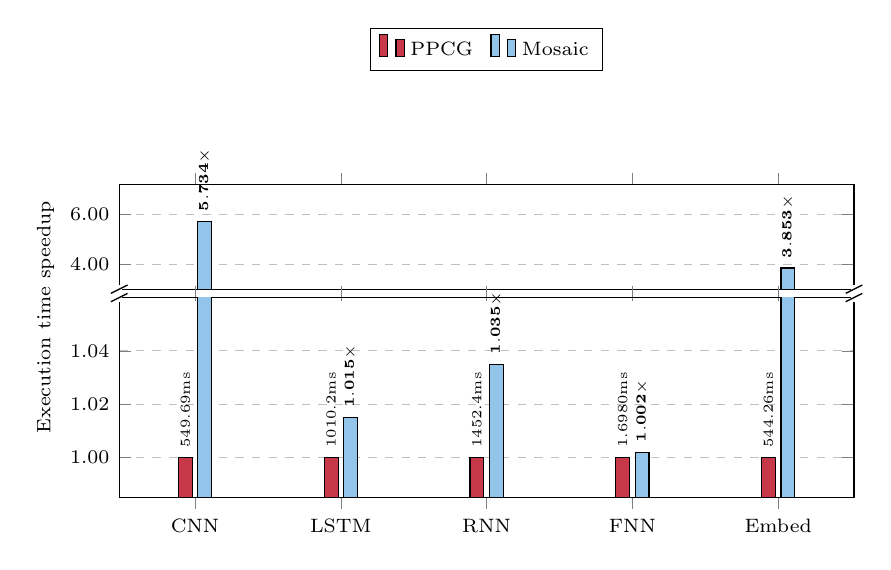
\begin{tikzpicture}
\begin{groupplot}[
    group style={
        group size=1 by 2,
        vertical sep=3pt,
        xticklabels at=edge bottom,
    },
    ybar,
    /pgf/bar width=5pt,        
    width=0.9\columnwidth,
    symbolic x coords={CNN,LSTM,RNN,FNN,Embed},
    xtick=data,
    enlarge x limits=0.13,
    ymajorgrids=true,
    grid style=dashed,
    xticklabel style={font=\scriptsize, text depth=0pt},
    yticklabel style={font=\scriptsize},
    nodes near coords,
    every node near coord/.append style={font=\tiny, rotate=90, anchor=west},
    point meta=explicit symbolic,
]

\nextgroupplot[
    height=0.24\columnwidth,
    ymin=3, ymax=7.2,
    ytick={4.00,6.00}, yticklabels={4.00,6.00},
    legend style={
        at={(0.5,2.5)}, anchor=north,
        legend columns=2, font=\scriptsize,
        /tikz/every even column/.append style={column sep=0.15cm},
    },
]
\addplot[fill=color1, draw=black] coordinates {
    (CNN,1)[] (LSTM,1)[] (RNN,1)[] (FNN,1)[] (Embed,1)[]
};
\addplot[fill=color4, draw=black] coordinates {
    (CNN,5.734)[$\mathbf{5.734}\mathbf{\times}$] (LSTM,1.015)[] (RNN,1.035)[] (FNN,1.002)[] (Embed,3.853)[$\mathbf{3.853}\mathbf{\times}$]
};
\legend{PPCG, Mosaic}

\nextgroupplot[
    height=0.34\columnwidth,
    ymin=0.985, ymax=1.06,
    ytick={1.00,1.02,1.04}, yticklabels={1.00,1.02,1.04},
]
\addplot[fill=color1, draw=black] coordinates {
    (CNN,1)[549.69ms] (LSTM,1)[1010.2ms] (RNN,1)[1452.4ms] (FNN,1)[1.6980ms] (Embed,1)[544.26ms]
};
\addplot[fill=color4, draw=black] coordinates {
    (CNN,5.734)[] (LSTM,1.015)[$\mathbf{1.015}\mathbf{\times}$] (RNN,1.035)[$\mathbf{1.035}\mathbf{\times}$] (FNN,1.002)[$\mathbf{1.002}\mathbf{\times}$] (Embed,3.853)[]
};
\end{groupplot}


\coordinate (bl) at ($(group c1r1.south west)!0.5!(group c1r2.north west)$);
\coordinate (br) at ($(group c1r1.south east)!0.5!(group c1r2.north east)$);
\foreach \p in {bl,br}{
    \draw[white,line width=2pt] ($(\p)+(0,-3pt)$)--($(\p)+(0,3pt)$);
    \draw[line width=.5pt] ($(\p)+(-3pt,-3pt)$)--($(\p)+(3pt,0pt)$);
    \draw[line width=.5pt] ($(\p)+(-3pt,0pt)$)--($(\p)+(3pt,3pt)$);
}


\node[rotate=90, anchor=south, font=\scriptsize]
    at ([xshift=-20pt]$(group c1r1.west)!0.5!(group c1r2.west)$)
    {Execution time speedup};
\end{tikzpicture}
\caption{Performance of deep learning operators.}
\Description{Bar chart comparing PPCG and \name speedups on CNN, LSTM, RNN, FNN, and embedding operators.}
\label{fig:network-operators}
\end{figure}

These operators cover different execution regimes. CNN and FNN are contraction/GEMM-like and therefore compute-intensive, but FNN is small and regular enough that the PPCG default already lands close to the configuration selected by \name. LSTM, in contrast, is a representative memory-intensive recurrent operator; its performance is dominated more by data movement than by arithmetic intensity, leaving less room for the register-blocking trade-offs captured by the $\phi$ ratio. Embedding is also data-movement dominated, but its default PPCG mapping leaves substantial opportunity for \name's placement and occupancy model to improve the execution configuration.

To compare \name against search-based autotuning, we integrate it into TVM~\cite{tvm} and compare with MetaSchedule~\cite{metaschedule} across trial budgets. \autoref{fig:network-operator-curves} plots execution time and selection cost for six operators. \name is flat because it solves once, whereas MetaSchedule needs hundreds to thousands of trials to reach comparable execution time and pays search cost that grows with the budget. \name therefore attains autotuner-level performance while reducing selection overhead by \(2\)--\(4\) orders of magnitude.

\begin{figure}[!tbp]
\centering
\definecolor{curveMosaic}{HTML}{CC0000}
\definecolor{curveTVM}{HTML}{FF6666}
\definecolor{curveSolverMosaic}{HTML}{0066CC}
\definecolor{curveSolverTVM}{HTML}{4D94E6}
\begin{tikzpicture}
\begin{scope}[xshift=0.1\columnwidth, yshift=4.55cm]
\begin{axis}[
    width=0.45\columnwidth, height=2.35cm,
    yticklabel style={color=curveMosaic, font=\scriptsize},
    ymode=log,
    ymin=1, ymax=100,
    ytick={1,10,100},
    xmode=log,
    xmin=0.8, xmax=1200,
    xtick={1,10,100,1000},
    xticklabels={1,$10^1$,$10^2$,$10^3$},
    xticklabel style={font=\scriptsize},
    grid=major,
    grid style={line width=0.3pt, draw=gray!25},
    axis y line*=left,
    axis x line*=bottom,
    title={CNN},
    title style={font=\footnotesize, yshift=-0.2cm},
]
\addplot[color=curveMosaic, line width=0.55pt, solid, mark=*, mark size=1.2pt] coordinates {
    (1,4.2312) (10,4.2312) (100,4.2312) (200,4.2312) (500,4.2312) (1000,4.2312)
};
\addplot[color=curveTVM, line width=0.55pt, solid, mark=square*, mark size=1.2pt] coordinates {
    (1,51.732) (10,60.3056) (100,6.7591) (200,6.8391) (500,7.4544) (1000,5.8638)
};
\end{axis}
\begin{axis}[
    width=0.45\columnwidth, height=2.35cm,
    axis y line*=right,
    axis x line=none,
    yticklabel style={color=curveSolverMosaic, opacity=0},
    ymode=log,
    ymin=0.1, ymax=1000,
    ytick={0.1,10,1000},
    xmode=log,
    xmin=0.8, xmax=1200,
]
\addplot[color=curveSolverMosaic, line width=0.55pt, dashed, mark=*, mark size=1.2pt] coordinates {
    (1,2.9676) (10,2.9676) (100,2.9676) (200,2.9676) (500,2.9676) (1000,2.9676)
};
\addplot[color=curveSolverTVM, line width=0.55pt, dashed, mark=square*, mark size=1.2pt] coordinates {
    (1,17.2) (10,42.3) (100,737.7) (200,939.3) (500,924.3) (1000,1078)
};
\end{axis}
\end{scope}

\begin{scope}[xshift=0.55\columnwidth, yshift=4.55cm]
\begin{axis}[
    width=0.45\columnwidth, height=2.35cm,
    yticklabel style={color=curveMosaic, font=\scriptsize},
    ymode=log,
    ymin=0.1, ymax=100,
    ytick={0.1,1,10},
    xmode=log,
    xmin=0.8, xmax=1200,
    xtick={1,10,100,1000},
    xticklabels={1,$10^1$,$10^2$,$10^3$},
    xticklabel style={font=\scriptsize},
    grid=major,
    grid style={line width=0.3pt, draw=gray!25},
    axis y line*=left,
    axis x line*=bottom,
    title={LSTM},
    title style={font=\footnotesize, yshift=-0.2cm},
]
\addplot[color=curveMosaic, line width=0.55pt, solid, mark=*, mark size=1.2pt] coordinates {
    (1,0.2332) (10,0.2332) (100,0.2332) (200,0.2332) (500,0.2332) (1000,0.2332)
};
\addplot[color=curveTVM, line width=0.55pt, solid, mark=square*, mark size=1.2pt] coordinates {
    (1,21.9229) (10,1.5843) (100,0.2814) (200,0.3319) (500,0.2185) (1000,0.2185)
};
\end{axis}
\begin{axis}[
    width=0.45\columnwidth, height=2.35cm,
    axis y line*=right,
    axis x line=none,
    yticklabel style={color=curveSolverMosaic, font=\scriptsize},
    ymode=log,
    ymin=0.01, ymax=2000,
    ytick={0.01,10,1000},
    xmode=log,
    xmin=0.8, xmax=1200,
]
\addplot[color=curveSolverMosaic, line width=0.55pt, dashed, mark=*, mark size=1.2pt] coordinates {
    (1,0.0741) (10,0.0741) (100,0.0741) (200,0.0741) (500,0.0741) (1000,0.0741)
};
\addplot[color=curveSolverTVM, line width=0.55pt, dashed, mark=square*, mark size=1.2pt] coordinates {
    (1,16) (10,22.47) (100,131.84) (200,267.54) (500,660.27) (1000,1326.86)
};
\end{axis}
\end{scope}

\begin{scope}[xshift=0.1\columnwidth, yshift=3cm]
\begin{axis}[
    width=0.45\columnwidth, height=2.35cm,
    yticklabel style={color=curveMosaic, font=\scriptsize},
    ymode=log,
    ymin=10, ymax=3000,
    ytick={10,100,1000},
    xmode=log,
    xmin=0.8, xmax=1200,
    xtick={1,10,100,1000},
    xticklabels={1,$10^1$,$10^2$,$10^3$},
    xticklabel style={font=\scriptsize},
    grid=major,
    grid style={line width=0.3pt, draw=gray!25},
    axis y line*=left,
    axis x line*=bottom,
    title={RNN},
    title style={font=\footnotesize, yshift=-0.2cm},
]
\addplot[color=curveMosaic, line width=0.55pt, solid, mark=*, mark size=1.2pt] coordinates {
    (1,20.4271) (10,20.4271) (100,20.4271) (200,20.4271) (500,20.4271) (1000,20.4271)
};
\addplot[color=curveTVM, line width=0.55pt, solid, mark=square*, mark size=1.2pt] coordinates {
    (1,2252.1594) (10,81.9091) (100,21.8536) (200,20.0876) (500,17.8522) (1000,17.7766)
};
\end{axis}
\begin{axis}[
    width=0.45\columnwidth, height=2.35cm,
    axis y line*=right,
    axis x line=none,
    yticklabel style={color=curveSolverMosaic, opacity=0},
    ymode=log,
    ymin=0.1, ymax=2000,
    ytick={0.1,10,1000},
    xmode=log,
    xmin=0.8, xmax=1200,
]
\addplot[color=curveSolverMosaic, line width=0.55pt, dashed, mark=*, mark size=1.2pt] coordinates {
    (1,0.716) (10,0.716) (100,0.716) (200,0.716) (500,0.716) (1000,0.716)
};
\addplot[color=curveSolverTVM, line width=0.55pt, dashed, mark=square*, mark size=1.2pt] coordinates {
    (1,23.44) (10,219.66) (100,823.3) (200,895.68) (500,1007.83) (1000,1012.12)
};
\end{axis}
\end{scope}

\begin{scope}[xshift=0.55\columnwidth, yshift=3cm]
\begin{axis}[
    width=0.45\columnwidth, height=2.35cm,
    yticklabel style={color=curveMosaic, font=\scriptsize},
    ymode=log,
    ymin=0.05, ymax=2,
    ytick={0.05,0.2,1},
    xmode=log,
    xmin=0.8, xmax=1200,
    xtick={1,10,100,1000},
    xticklabels={1,$10^1$,$10^2$,$10^3$},
    xticklabel style={font=\scriptsize},
    grid=major,
    grid style={line width=0.3pt, draw=gray!25},
    axis y line*=left,
    axis x line*=bottom,
    title={FNN},
    title style={font=\footnotesize, yshift=-0.2cm},
]
\addplot[color=curveMosaic, line width=0.55pt, solid, mark=*, mark size=1.2pt] coordinates {
    (1,0.0738) (10,0.0738) (100,0.0738) (200,0.0738) (500,0.0738) (1000,0.0738)
};
\addplot[color=curveTVM, line width=0.55pt, solid, mark=square*, mark size=1.2pt] coordinates {
    (1,0.9439) (10,1.2417) (100,0.1618) (200,0.0944) (500,0.081) (1000,0.0741)
};
\end{axis}
\begin{axis}[
    width=0.45\columnwidth, height=2.35cm,
    axis y line*=right,
    axis x line=none,
    yticklabel style={color=curveSolverMosaic, font=\scriptsize},
    ymode=log,
    ymin=0.01, ymax=1000,
    ytick={0.01,1,100},
    xmode=log,
    xmin=0.8, xmax=1200,
]
\addplot[color=curveSolverMosaic, line width=0.55pt, dashed, mark=*, mark size=1.2pt] coordinates {
    (1,0.1194) (10,0.1194) (100,0.1194) (200,0.1194) (500,0.1194) (1000,0.1194)
};
\addplot[color=curveSolverTVM, line width=0.55pt, dashed, mark=square*, mark size=1.2pt] coordinates {
    (1,9.8) (10,15.2) (100,78.2) (200,122.8) (500,282.5) (1000,561.9)
};
\end{axis}
\end{scope}

\begin{scope}[xshift=0.1\columnwidth, yshift=1.4cm]
\begin{axis}[
    width=0.45\columnwidth, height=2.35cm,
    yticklabel style={color=curveMosaic, font=\scriptsize},
    ymode=log,
    ymin=10, ymax=500,
    ytick={10,50,200},
    xmode=log,
    xmin=0.8, xmax=1200,
    xtick={1,10,100,1000},
    xticklabels={1,$10^1$,$10^2$,$10^3$},
    xticklabel style={font=\scriptsize},
    grid=major,
    grid style={line width=0.3pt, draw=gray!25},
    axis y line*=left,
    axis x line*=bottom,
    title={Embedding},
    title style={font=\footnotesize, yshift=-0.2cm},
]
\addplot[color=curveMosaic, line width=0.55pt, solid, mark=*, mark size=1.2pt] coordinates {
    (1,12.9526) (10,12.9526) (100,12.9526) (200,12.9526) (500,12.9526) (1000,12.9526)
};
\addplot[color=curveTVM, line width=0.55pt, solid, mark=square*, mark size=1.2pt] coordinates {
    (1,362.8838) (10,85.9239) (100,38.2759) (200,32.3857) (500,29.9019) (1000,25.491)
};
\end{axis}
\begin{axis}[
    width=0.45\columnwidth, height=2.35cm,
    axis y line*=right,
    axis x line=none,
    yticklabel style={color=curveSolverMosaic, opacity=0},
    ymode=log,
    ymin=0.01, ymax=3000,
    ytick={0.01,10,1000},
    xmode=log,
    xmin=0.8, xmax=1200,
]
\addplot[color=curveSolverMosaic, line width=0.55pt, dashed, mark=*, mark size=1.2pt] coordinates {
    (1,0.3567) (10,0.3567) (100,0.3567) (200,0.3567) (500,0.3567) (1000,0.3567)
};
\addplot[color=curveSolverTVM, line width=0.55pt, dashed, mark=square*, mark size=1.2pt] coordinates {
    (1,16.71) (10,108.89) (100,610.7) (200,1041.74) (500,2432.51) (1000,2432.51)
};
\end{axis}
\end{scope}

\begin{scope}[xshift=0.55\columnwidth, yshift=1.4cm]
\begin{axis}[
    width=0.45\columnwidth, height=2.35cm,
    yticklabel style={color=curveMosaic, font=\scriptsize},
    ymode=log,
    ymin=1, ymax=50,
    ytick={1,5,20},
    xmode=log,
    xmin=0.8, xmax=1200,
    xtick={1,10,100,1000},
    xticklabels={1,$10^1$,$10^2$,$10^3$},
    xticklabel style={font=\scriptsize},
    grid=major,
    grid style={line width=0.3pt, draw=gray!25},
    axis y line*=left,
    axis x line*=bottom,
    title={Matmul},
    title style={font=\footnotesize, yshift=-0.2cm},
]
\addplot[color=curveMosaic, line width=0.55pt, solid, mark=*, mark size=1.2pt] coordinates {
    (1,4.4347) (10,4.4347) (100,4.4347) (200,4.4347) (500,4.4347) (1000,4.4347)
};
\addplot[color=curveTVM, line width=0.55pt, solid, mark=square*, mark size=1.2pt] coordinates {
    (1,26.5995) (10,20.8549) (100,7.149) (200,4.2035) (500,4.5826) (1000,4.1599)
};
\end{axis}
\begin{axis}[
    width=0.45\columnwidth, height=2.35cm,
    axis y line*=right,
    axis x line=none,
    yticklabel style={color=curveSolverMosaic, font=\scriptsize},
    ymode=log,
    ymin=0.01, ymax=2000,
    ytick={0.01,10,1000},
    xmode=log,
    xmin=0.8, xmax=1200,
]
\addplot[color=curveSolverMosaic, line width=0.55pt, dashed, mark=*, mark size=1.2pt] coordinates {
    (1,0.21) (10,0.21) (100,0.21) (200,0.21) (500,0.21) (1000,0.21)
};
\addplot[color=curveSolverTVM, line width=0.55pt, dashed, mark=square*, mark size=1.2pt] coordinates {
    (1,11.06) (10,88.17) (100,360.63) (200,601.6) (500,866.03) (1000,1671.5)
};
\end{axis}
\end{scope}

\node[rotate=90, color=curveMosaic, font=\scriptsize] at (0\columnwidth, 3.38cm) {Execution time (ms)};
\node[rotate=90, color=curveSolverMosaic, font=\scriptsize] at (0.91\columnwidth, 3.38cm) {Search/solver (s)};
\node[font=\scriptsize] at (0.47\columnwidth, 0.80cm) {Number of Trials};
\node at (0.48\columnwidth, 0.42cm) {
    \begin{tikzpicture}
        % Mosaic exec.
        \draw[color=curveMosaic, line width=0.7pt, solid] (0,0) -- (0.28,0);
        \filldraw[fill=curveMosaic, draw=white, line width=0.3pt]
            (0.16,0) circle (0.045);
        \node[right, font=\tiny] at (0.34,0) {Mosaic exec.};

        % TVM exec.
        \draw[color=curveTVM, line width=0.7pt, solid] (1.57,0) -- (1.85,0);
        \filldraw[fill=curveTVM, draw=white, line width=0.3pt]
            (1.68,-0.05) rectangle (1.78,0.05);
        \node[right, font=\tiny] at (1.89,0) {TVM exec.};

        % Mosaic solver
        \draw[color=curveSolverMosaic, line width=0.7pt, dashed] (3.00,0) -- (3.28,0);
        \filldraw[fill=curveSolverMosaic, draw=white, line width=0.3pt]
            (3.16,0) circle (0.045);
        \node[right, font=\tiny] at (3.34,0) {Mosaic solver};

        % TVM search
        \draw[color=curveSolverTVM, line width=0.7pt, dashed] (4.75,0) -- (5.03,0);
        \filldraw[fill=curveSolverTVM, draw=white, line width=0.3pt]
            (4.86,-0.05) rectangle (4.96,0.05);
        \node[right, font=\tiny] at (5.09,0) {TVM search};
    \end{tikzpicture}
};

\end{tikzpicture}
\caption{Execution time and search/solver overhead for six operators, comparing with TVM MetaSchedule. Solid lines show execution time; dashed lines show selection cost.}
\Description{Six curve plots for CNN, LSTM, RNN, FNN, embedding, and matmul comparing \name and tvm SSSRRSRS execution time and search or solver overhead.}
\label{fig:network-operator-curves}
\end{figure}

\subsection{Performance on End-to-End Workloads}
\label{subsec:e2e}

We compose the operators into three end-to-end workloads spanning the major network families: AlexNet~\cite{alexnet} (CNN), Seq2Seq~\cite{lstm} (RNN), and BertTiny~\cite{bert} (Transformer). \autoref{fig:e2e-fourbar} reports the per-network speedup of \name over both PPCG and TVM, with the baseline execution times shown on the left of the corresponding bars. Over PPCG, \name achieves $1.66\times$, $9.23\times$, and $4.90\times$ on AlexNet, Seq2Seq, and BertTiny, respectively, for a mean speedup of $4.22\times$. Over TVM MetaSchedule, \name achieves $1.16\times$, $1.05\times$, and $1.13\times$, for a mean of $1.11\times$. These results demonstrate that \name slightly exceeds a state-of-the-art autotuner on full workloads without performing any architecture-space search, while delivering large improvements over the heuristic configurations of PPCG. The end-to-end gains over PPCG are more pronounced than the per-operator gains of \autoref{subsec:operators}, as consistently good execution space choices across consecutive layers compound into a larger overall improvement.

\begin{figure}[htbp]
\centering
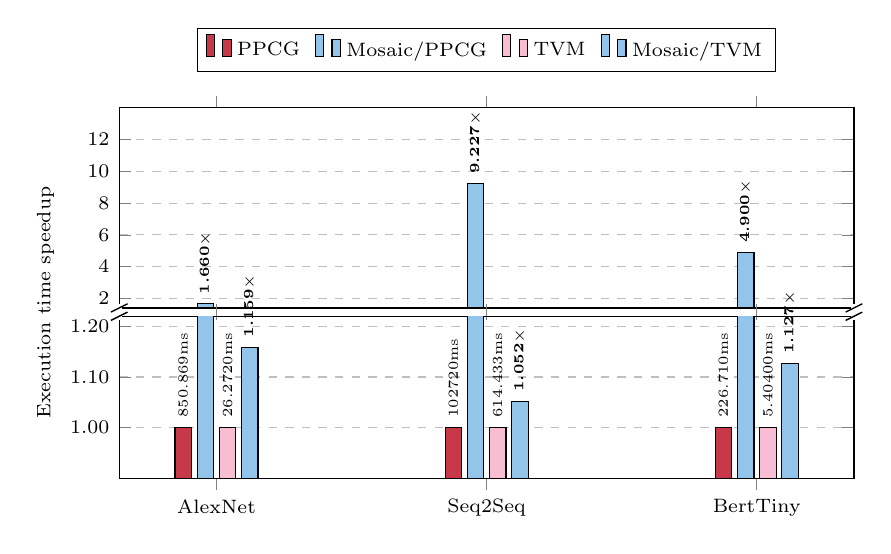
\begin{tikzpicture}
\begin{groupplot}[
    group style={
        group size=1 by 2,
        vertical sep=3pt,
        xticklabels at=edge bottom,
    },
    ybar,
    /pgf/bar width=6pt,
    width=0.9\columnwidth,
    symbolic x coords={AlexNet,Seq2Seq,BertTiny},
    xtick=data,
    enlarge x limits=0.18,
    ymajorgrids=true,
    grid style=dashed,
    xticklabel style={font=\scriptsize},
    yticklabel style={font=\scriptsize},
    nodes near coords,
    every node near coord/.append style={font=\tiny, rotate=90, anchor=west},
    point meta=explicit symbolic,
]

\nextgroupplot[
    height=0.34\columnwidth,
    ymin=1.4, ymax=14,
    ytick={2,4,6,8,10,12}, yticklabels={2,4,6,8,10,12},
    legend style={at={(0.5,1.18)}, anchor=south, legend columns=4, font=\scriptsize,
        /tikz/every even column/.append style={column sep=0.12cm}},
]
\addplot[fill=color1,draw=black] coordinates {(AlexNet,1)[] (Seq2Seq,1)[] (BertTiny,1)[]};
\addplot[fill=color4,draw=black] coordinates {(AlexNet,1.660)[\textbf{1.660$\times$}] (Seq2Seq,9.227)[\textbf{9.227$\times$}] (BertTiny,4.900)[\textbf{4.900$\times$}]};
\addplot[fill=color2,draw=black] coordinates {(AlexNet,1)[] (Seq2Seq,1)[] (BertTiny,1)[]};
\addplot[fill=color4,draw=black] coordinates {(AlexNet,1.159)[] (Seq2Seq,1.052)[] (BertTiny,1.127)[]};
\legend{PPCG, \name/PPCG, TVM, \name/TVM}

\nextgroupplot[
    height=0.30\columnwidth,
    ymin=0.9, ymax=1.22,
    ytick={1.00,1.10,1.20}, yticklabels={1.00,1.10,1.20},
]
\addplot[fill=color1,draw=black] coordinates {(AlexNet,1)[850.869ms] (Seq2Seq,1)[102720ms] (BertTiny,1)[226.710ms]};
\addplot[fill=color4,draw=black] coordinates {(AlexNet,1.660)[] (Seq2Seq,9.227)[] (BertTiny,4.900)[]};
\addplot[fill=color2,draw=black] coordinates {(AlexNet,1)[26.2720ms] (Seq2Seq,1)[614.433ms] (BertTiny,1)[5.40400ms]};
\addplot[fill=color4,draw=black] coordinates {(AlexNet,1.159)[\textbf{1.159$\times$}] (Seq2Seq,1.052)[\textbf{1.052$\times$}] (BertTiny,1.127)[\textbf{1.127$\times$}]};
\end{groupplot}
 

\coordinate (bl) at ($(group c1r1.south west)!0.5!(group c1r2.north west)$);
\coordinate (br) at ($(group c1r1.south east)!0.5!(group c1r2.north east)$);
\foreach \p in {bl,br}{
    \draw[white,line width=2pt] ($(\p)+(0,-3pt)$)--($(\p)+(0,3pt)$);
    \draw[line width=.5pt] ($(\p)+(-3pt,-3pt)$)--($(\p)+(3pt,0pt)$);
    \draw[line width=.5pt] ($(\p)+(-3pt,0pt)$)--($(\p)+(3pt,3pt)$);
}
\node[rotate=90, anchor=south, font=\scriptsize]
    at ([xshift=-20pt]$(group c1r1.west)!0.5!(group c1r2.west)$) {Execution time speedup};
\end{tikzpicture}
\caption{Performance of end-to-end workloads.}
\Description{Four bars per network: PPCG baseline, \name over PPCG, TVM baseline, and \name over TVM.}
\label{fig:e2e-fourbar}
\end{figure}

\subsection{Ablation Study}
\label{subsec:ablation}

We ablate the main modeling components on representative kernels and operators. FP-Wave uses the quantized wave objective with a fixed placement; RF-Wave adds the conservative register-feasibility filter; the full \name model further enumerates shared memory placement schemes. Using FP-Wave as the baseline, RF-Wave improves performance by a  mean of $1.37\times$, while full \name reaches $1.84\times$. The largest gain comes on CNN, where register filtering and placement selection together improve the selected configuration from $265.793$~ms to $95.851$~ms.

\begin{figure}[htbp]
\centering
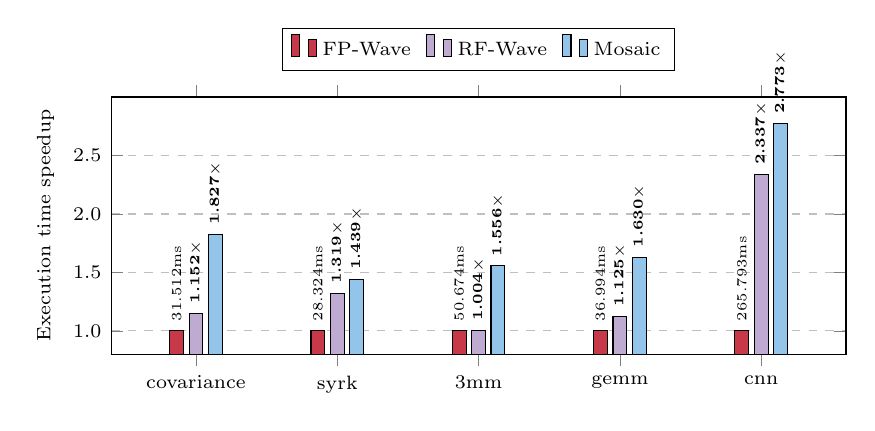
\begin{tikzpicture}
\begin{axis}[
    ybar,
    /pgf/bar width=5pt,
    width=0.9\columnwidth,
    height=0.40\columnwidth,
    symbolic x coords={covariance,syrk,3mm,gemm,cnn},
    xtick=data,
    enlarge x limits=0.15,
    ymin=0.8,
    ymax=3.0,
    ytick={1.0,1.5,2.0,2.5},
    yticklabels={1.0,1.5,2.0,2.5},
    ymajorgrids=true,
    grid style=dashed,
    xticklabel style={font=\scriptsize},
    yticklabel style={font=\scriptsize},
    ylabel={Execution time speedup},
    ylabel style={font=\scriptsize},
    nodes near coords,
    every node near coord/.append style={font=\tiny, rotate=90, anchor=west},
    point meta=explicit symbolic,
    legend style={
        at={(0.5,1.10)}, anchor=south,
        legend columns=3, font=\scriptsize,
        /tikz/every even column/.append style={column sep=0.12cm}
    },
]
\addplot[fill=color1, draw=black] coordinates {
    (covariance,1)[31.512ms]
    (syrk,1)[28.324ms]
    (3mm,1)[50.674ms]
    (gemm,1)[36.994ms]
    (cnn,1)[265.793ms]
};
\addplot[fill=color3, draw=black] coordinates {
    (covariance,1.152)[\textbf{1.152$\times$}]
    (syrk,1.319)[\textbf{1.319$\times$}]
    (3mm,1.004)[\textbf{1.004$\times$}]
    (gemm,1.125)[\textbf{1.125$\times$}]
    (cnn,2.337)[\textbf{2.337$\times$}]
};
\addplot[fill=color4, draw=black] coordinates {
    (covariance,1.827)[\textbf{1.827$\times$}]
    (syrk,1.439)[\textbf{1.439$\times$}]
    (3mm,1.556)[\textbf{1.556$\times$}]
    (gemm,1.630)[\textbf{1.630$\times$}]
    (cnn,2.773)[\textbf{2.773$\times$}]
};
\legend{FP-Wave, RF-Wave, Mosaic}
\end{axis}
\end{tikzpicture}
\caption{Ablation study on \name's individual components.}
\Description{Grouped bar chart showing execution-time speedups of RF-Wave and Mosaic over the FP-Wave baseline on covariance, syrk, 3mm, gemm, and CNN.}
\label{fig:ablation}
\end{figure}

\subsection{Solver Overhead and Scalability}
\label{subsec:overhead}

Finally, we examine the cost of \name's analytical selection, reported in the solver-time columns of \autoref{tab:benchmark}. \name completes its two-stage solving in well under one second for the large majority of kernels and in at most a few seconds in the most demanding case (e.g., \texttt{syr2k} at $3.32$~s on the RTX 4090), since the feasible domain is bounded by the guard-free candidate sets of \autoref{sec:abstraction} and pruned by the conservative filters of \autoref{sec:constraints} before the MILP is ever invoked. Relative to EATSS, \name reduces selection overhead by mean factors of $12.6\times$, $13.6\times$, and $13.9\times$ on RTX 4090, A100, and V100, respectively, and the gap relative to the trial-based search of TVM spans several orders of magnitude (\autoref{fig:network-operator-curves}). As with the per-architecture profile, this selection cost is a one-time, compile-time expense that no runtime tuning loop contributes to, confirming that \name's analytical formulation scales to large, real-world kernels and workloads.

% !TEX root =  mosaic.tex
\section{Related Work}
\label{sec:related}

GPU execution-space selection is dominated by fixed heuristics and empirical
search, while analytical decoupled selection has been developed mostly for CPUs.
\name carries that lineage to GPUs by modeling the feedback loop of
\autoref{sec:bg-challenges} directly.

Polyhedral GPU code generation derives transformations and emits accelerator
code.
PPCG~\cite{ppcg} is the de-facto polyhedral GPU back-end, but fixes tile sizes
and launches by heuristic rules; later mapping work such as hybrid
hexagonal/classical tiling for stencils~\cite{hybridtile} still leaves these
parameters to policy. \name performs no scheduling: it consumes the transformed
program and optimizes only the execution-space decisions.

Tile-size selection began with CPU cache models~\cite{mckinley-tss,lam-tss};
later systems embed polynomial or geometric
programming in compilers~\cite{pluto-tss,pluto,rajopadhye-gp,rajopadhye-igp}.
TileMind~\cite{tilemind} decouples the selector as a MILP over compile-time
metadata and profiled CPU costs. These systems rely on separable residency:
footprint \(\le\) capacity. On GPUs, a tile also changes shared memory
footprint, register working set, occupancy, and wave count. \name therefore
replaces CPU residency with quantized wave cost and a conservative register
filter.

Among analytical models for GPUs, EATSS~\cite{eatss} is an analytical GPU
tile-size selector embedded in PPCG, but is compiler-coupled and narrower.
Kernel-specific GPU models cover GEMM and
convolution~\cite{li-gemm,blis,saday-conv}; \name instead spans reductions,
contractions, and stencils through \(\phi\) and explicitly models
occupancy--register coupling and wave quantization.

Search-based autotuning systems such as TVM, Ansor, and
MetaSchedule~\cite{tvm,ansor,metaschedule}
generate and time configurations, achieving high performance at substantial
tuning cost. Hybrid and learning-based approaches prune or approximate this
search~\cite{shirako-tss,hctuner,yuki-tss}, often under restricted tile spaces.
\name instead derives interpretable configurations analytically.

% !TEX root =  mosaic.tex
\section{Conclusion}
\label{sec:conclusion}

We presented \name, a unified analytical framework for GPU execution-space optimization. \name selects tile sizes and thread-block dimensions for a transformed program whose schedule is already fixed, reasoning over abstract shared-memory placement scenarios. Its two-stage analytical selection preserves the quantized primary optimum and uses a relaxed-cost tie-break only among tied legal discrete configurations, including across modeled placement scenarios, so \name selects these parameters without generating and evaluating large numbers of GPU kernels. Experimental results include a cross-generation PolyBench evaluation on three NVIDIA GPUs, together with deep learning operators and end-to-end workloads on the RTX 4090. Across these experiments, \name achieves geometric-mean speedups over PPCG, lower aggregate latency relative to EATSS, and slightly higher end-to-end performance than TVM MetaSchedule at substantially lower optimization overhead, suggesting that architecture-aware execution-space optimization can be addressed analytically rather than through measurement-driven search.

\name operates after transformation scheduling: it preserves the upstream schedule and mapping structure, selects tile and thread-block parameters, and leaves concrete shared-memory staging to the backend. Its cost model uses the loop and access metadata of \autoref{sec:metadata} and covers conventional CUDA-core SIMT execution, as evaluated through the PPCG and non-tensorized TVM paths. It stops there: tensor-core operand staging and MMA shapes, asynchronous copy and the pipelines built on it, shared-memory swizzling, warp specialization, and thread-block clusters lie outside it, and where those mechanisms decide performance, the parameters \name selects are not the ones that decide it. What would carry over to such a target is the structure rather than the contents of the formulation: wave quantization follows from an SM hosting an integer number of blocks, and residency from the register and shared-memory budgets, neither of which depends on what issues the arithmetic. The terms would change: \(\phi\) would normalize operand reads by MMA tiles rather than by per-thread FMAs, \(\hat R\) would count accumulator fragments, and the \(\Lambda\) family would need constants for the asynchronous paths. Irregular accesses need metadata this interface does not carry.


\bibliographystyle{ACM-Reference-Format}
\bibliography{references}

% \appendix
% % !TEX root =  mosaic.tex
\section{Appendix}
\label{sec:appendix}

This appendix can include extended proofs, additional solver details, complete hardware parameters, workload descriptions, and supplementary evaluation results.


\end{document}
\endinput
